% !TEX root = ../lectures.tex
%%%%%%%%%% SECTION %%%%%%%%%
\section{Cosmic-ray protons in the Galaxy}
\label{sec:protons}

\begin{figure}[t]
\centering
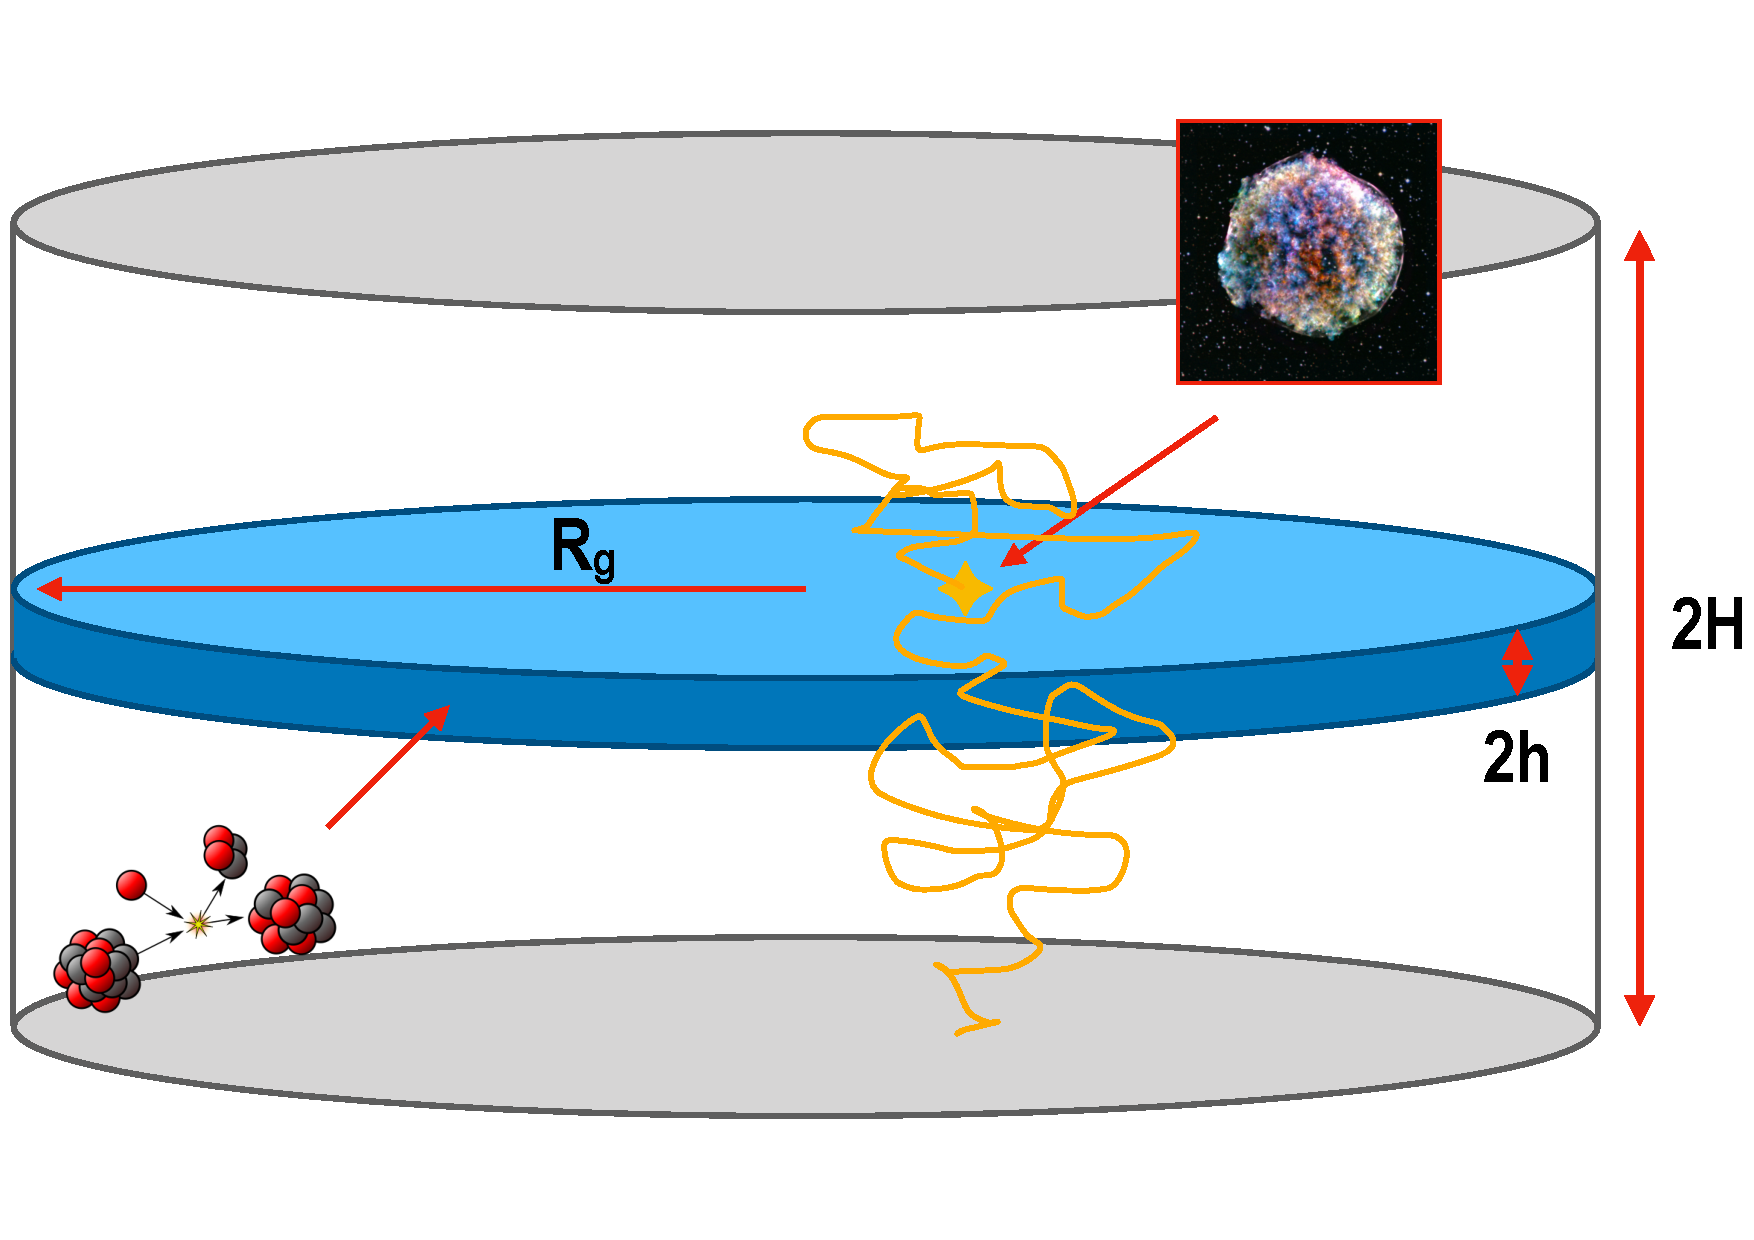
\includegraphics[width=0.6\textwidth]{figures/halo.pdf}
\caption{Illustrative depiction of the Milky Way's diffusive halo from the perspective of a cosmic ray physicist. Primary sources are distributed only in the disk. Also secondary nuclei emerge from cosmic ray interactions within the gaseous disk.}
\label{fig:galaxy}
\end{figure}

The local density of CRs, their energy spectrum, and their relative abundances provide us with the only direct information we can obtain about CRs. These measurements, along with estimates of the CR column density deduced from diffuse $\gamma$-rays~\cite{Tibaldo2021universe, Grenier2015araa}, form the foundation for any model aiming to describe CR transport.
%
In this section, our goal is to construct a basic model for CR propagation in the Galaxy that enables us to extract from these observables valuable information on the injection of CRs and the subsequent processes they undergo in the ISM.

As discussed in section~\ref{sec:pillar}, the escape time of CRs is too long to be compatible with straight propagation along the large-scale magnetic field. Consequently, CRs must be confined to the Galaxy for a significant period of time, primarily spending most of their time in low-density gas regions, such as the Galactic halo.
%
The existence of such an extended (larger than the gas disc) magnetized region is supported by observations of synchrotron emission from edge-on external galaxies~\cite{Beck2015aar}.

To account for these crucial aspects, virtually all CR transport models rely on the same basic ideas: high-energy particles are accelerated in sources located in a thin disc region of thickness $h \sim 100$ pc, following an injected spectrum proportional to $E^{-\gamma}$, with $\gamma \gtrsim 2$ as expected in the presence of diffusive shock acceleration mechanism.

After the injection, CRs propagate diffusively throughout the Galactic halo, which has a scale height $H$ of approximately several kiloparsecs with a diffusion coefficient $D$ proportional to $E^\delta$, where $\delta \sim 1/3 - 1/2$, and they escape freely at the boundaries. The escape is an essential, yet poorly understood, process to guarantee the stationarity of the problem, and is usually simplified by setting the CR density to zero at the boundary $H$ above and below the Galactic plane~\cite{Ginzburg1980apss} (see figure~\ref{fig:galaxy}).

Since the size of the halo is much smaller than the Galaxy's radius ($R_{\rm d} \gtrsim 10$ kpc), a one-dimensional model is sufficient to describe the escape of CRs along the z-direction.

The simplest representation of this framework is achieved by employing the diffusion equation in the form of Fick's law~\cite{Fick1855}. 
%
It is important to note that one could also utilize the more general Fokker-Planck equation~\cite{Mertschreview?}.
%
Both Fick's law and the Fokker-Planck equation are considered as purely phenomenological equations, as they represent different choices for the flux in the fundamental continuity equation.

In general, we can write the continuity equation with a source term $Q(E, z)$ as
%
\begin{equation}
\frac{\partial n}{\partial t} + \frac{\partial J}{\partial z} = Q
\end{equation}
%
where $n(E, z, t)$ is the CR number density per unit energy and $J$ the corresponding flux along $z$.

According to Fick's law of diffusion, the diffusive flux is determined by the concentration gradient as $J = -D \nabla n$. In other words, a spatial gradient in the particle density will give rise to a current that transports particles from regions of high density to regions of low density, with the magnitude of the current being proportional to the diffusion coefficient $D$. The dimensions of $D$ are then \emph{area per unit time}.

The diffusion equation becomes
%
\begin{equation}
\frac{\partial n}{\partial t} = \frac{\partial}{\partial z} \left( D\frac{\partial n}{\partial z} \right) + Q
\end{equation}

For a spatially constant diffusion coefficient we can derive the associated Green’s function as 
%
\begin{equation}
\mathcal G(z,t) = \left(\frac{1}{{4 \pi D t}}\right)^{1/2} {\rm e}^{-\frac{z^2}{4Dt}}
\label{eq:green}
\end{equation}
%
which we interpret as the probability for finding a particle that is injected at the disc ($z = 0$) at a position $z$ after the time $t$.

\begin{figure}[t]
\centering
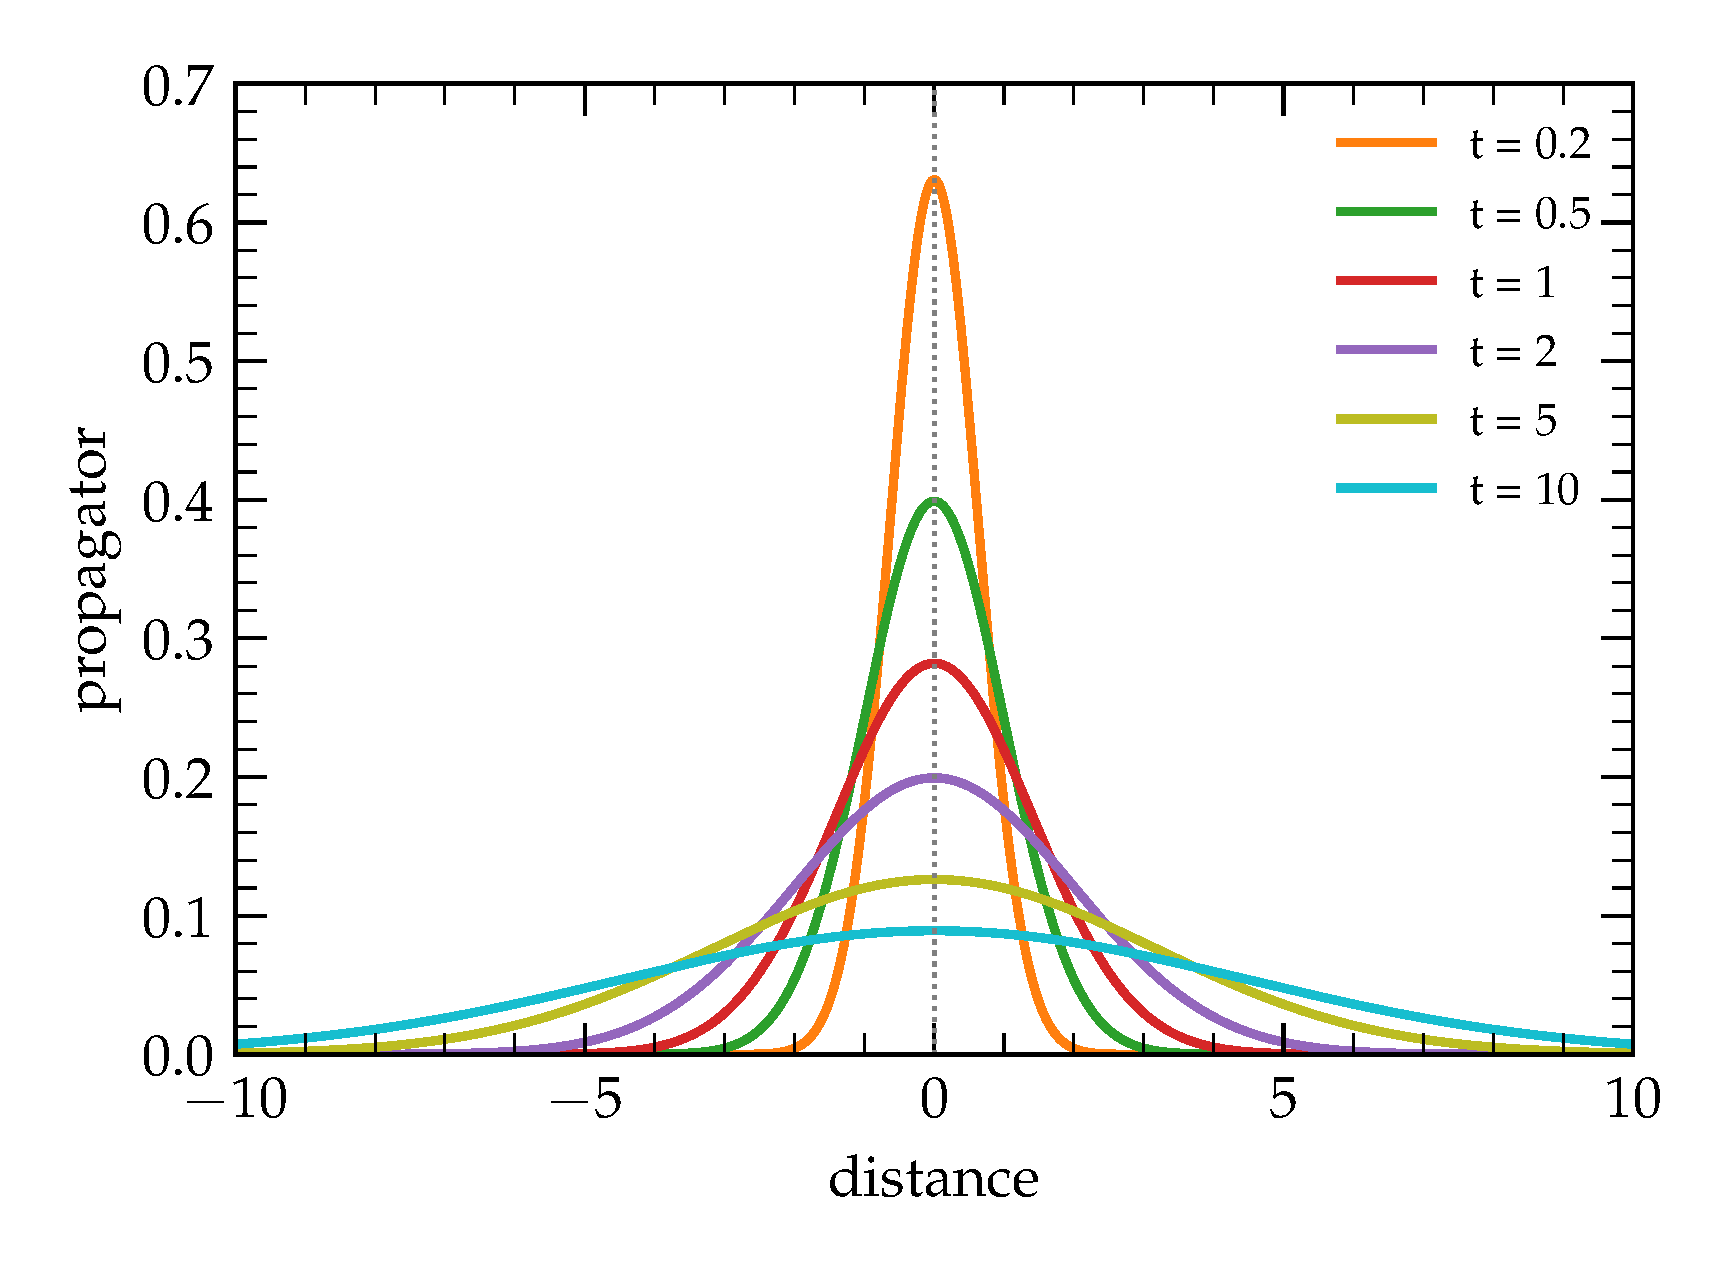
\includegraphics[width=0.6\textwidth]{figures/gaussian_1D.pdf} 
\caption{1D Gaussian propagator as a function of distance for various time steps. The plot demonstrates the spreading behavior of the diffusion Green function, \ref{eq:green}, with increasing time.}
\label{fig:gaussian1d}
\end{figure}

The mean distance from the Galactic plane can be calculated from~\ref{eq:green}:
%
\begin{equation}
\langle z \rangle = \left(\frac{1}{{4 \pi D t}}\right)^{1/2} \int dz z {\rm e}^{-\frac{z^2}{4Dt}} \simeq \sqrt{Dt}
\end{equation}

The characteristic time to reach a height $\langle z \rangle = H$ can then be defined as  $t_{\rm H} \simeq H^2 / D$, and the characteristic averaged velocity with which CRs escape from the Galaxy as the \emph{drift velocity}:
%
\begin{equation}
v_{\rm D} \sim \frac{H}{t_{\rm H}} \sim \frac{D}{H}
\end{equation}

It is important to acknowledge that in order to obtain the average distance from the galactic plane, we made the assumption that the diffusion coefficient remains spatially constant throughout both the halo and the disc. However, due to the variations in gas densities and magnetic field strengths between these regions, this assumption may not hold true.

By adopting the phenomenological assumption of diffusion as the primary transport process, we can construct the CR evolution equation by specifying the source term assuming Galactic Supernovae (SNe) as major contributors.

Since the galactic disc is extremely thin with respect to the halo, we can describe the spatial part of the injection term as a delta-function $\delta(z)$, and therefore
%
\begin{equation}\label{eq:qprotons}
Q(E,z) = \frac{\xi_{\rm CR} E_{\rm SN} \mathcal R_{\rm SN} N(E)}{\pi R_{\rm d}^2} \delta(z) 
\end{equation}
%
where $E_{\rm SN} \simeq 10^{51}$~erg is the SN kinetic energy, $\xi_{\rm CR}$ is the fraction of this energy converted in CR acceleration, $\mathcal R_{\rm SN} \simeq 1 / 50$~yr$^{-1}$ is the rate of SNe in the Galaxy and $N(E)$ the energy spectrum of one SN. 

Considering that our Galaxy has an age of several billion years and observations of light elements suggest that CRs spend at most a hundred million years within our Galaxy, it can be concluded that the dynamical timescale of the Galaxy is significantly longer than the phenomena we are investigating. Therefore, we are justified in assuming stationarity, and the diffusion equation for protons $n_p$ becomes:
%
\begin{equation}
-\frac{\partial}{\partial z}\left[ D(E) \frac{\partial n_p}{\partial z}\right] = \frac{\xi_p E_{\rm SN} \mathcal R_{\rm SN}}{\pi R_{\rm d}^2} N(E) \delta(z)
\label{eq:protons}
\end{equation}

For $z \ne 0$, and imposing the boundary conditions $n_p(z = \pm H, E) = 0$, it gives the solution\footnote{The general solution to the differential equation can be written as $n_p(z)=A+Bz$. For $z>0$, we impose $n_p(H)=0$ which gives $n_p(z)=A\left(1- z/H\right)$, and for $z<0$, we impose $n_{\rm p}(-H)=0$ which gives $n_{\rm p}(z)=A\left(1+ z/H\right)$. Combining the two regions and imposing $n_p(0)=n_0(E)$, we obtain the solution valid in both regions as in~\ref{eq:nzwithabs}.}:
%
\begin{equation}
D \frac{\partial n_p}{\partial z} = \text{Constant} \, \longrightarrow \, n_p(z) = n_0(E) \left( 1 - \frac{|z|}{H} \right)
\label{eq:nzwithabs}
\end{equation}

Thereby the diffusive flux is found to be constant in $z$, and we can compute it at the disc $z = 0$ as:
%
\begin{equation}
\left. D \frac{\partial n_p}{\partial z}\right|_{z=0^+} = - D \frac{n_{0}}{H}
\label{eq:flux}
\end{equation}

To find the density $n_0$ we integrate the diffusion equation around $z=0$:
%
\begin{equation}
\lim_{\epsilon\rightarrow0} \int_{\epsilon^-}^{\epsilon^+} \!\!\! dz 
\left\{ -\frac{\partial}{\partial z} \left[ D \frac{\partial n_p}{\partial z} \right] = Q(E,z) \right\} 
\end{equation}
%
which leads to
%
\begin{equation}
\left. -2D \frac{\partial n_p}{\partial z}\right|_{z=0^+} = \frac{\xi_p E_{\rm SN} \mathcal R_{\rm SN}}{\pi R_{\rm d}^2} N(E) 
\end{equation}
%
and using the equation for the flux derived in~\ref{eq:flux}:
%
\begin{equation}
n_p(E) = \frac{\xi_p E_{\rm SN} \mathcal R_{\rm SN} N(E)}{2 \pi R_{\rm d}^2}  \frac{H}{D(E)} 
\label{eq:protonsimplesolution}
\end{equation}

As a result, we have obtained the CR spectrum as measured by an observer placed within the galactic disc.
%
It can be simply re-written as:
%
\begin{remark}
\begin{equation}
n_p(E) = \frac{Q_{\rm SN}(E) \tau_{\rm esc}(E)}{V_{\rm G}}
\end{equation}
\end{remark}
%
where $Q_{\rm SN}(E) = \xi_p E_{\rm SN} \mathcal R_{\rm SN} N(E)$ is the number of particles injected per unit time by all supernovae, $\tau_{\rm esc} = H^2/D$ is the escape time, and $V_{\rm G} = 2\pi R_{\rm d}^2H$ is the total volume of the Galaxy.

\begin{figure}[t]
\centering
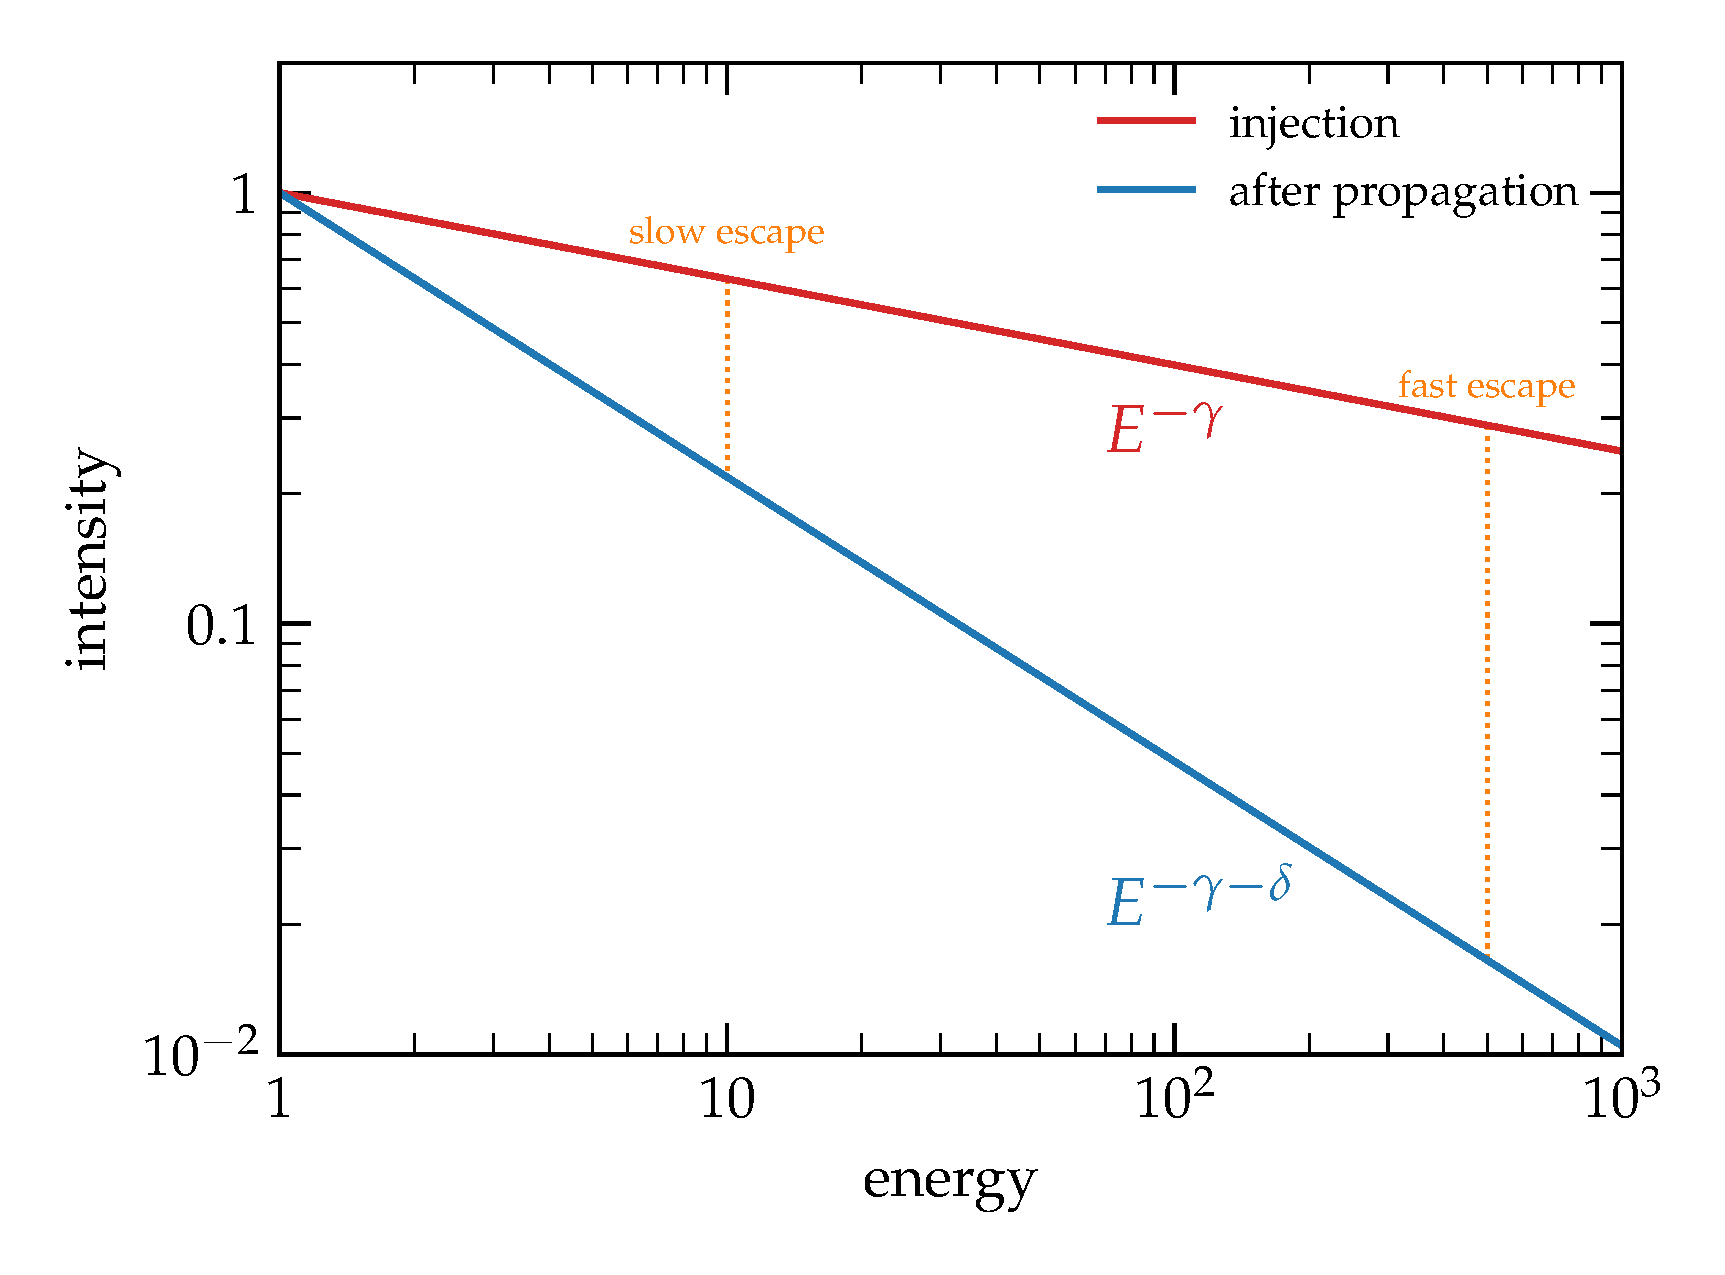
\includegraphics[width=0.6\textwidth]{figures/diffusion_softening.pdf}
\caption{Comparison between the \emph{injection spectrum} and the \emph{propagated spectrum} within an energy-dependent \emph{diffusion} model. Higher-energy particles escape more swiftly, leading to a reduced equilibrium intensity. Consequently, the propagated spectrum consistently exhibits a \emph{steeper} profile than the injected counterpart.}
\label{fig:softening}
\end{figure}

In summary, since the diffusion coefficient increases with energy, following a power-law dependence as $D \propto E^{\delta}$, the escape time scales $\tau_{\rm esc} \propto E^{-\delta}$, and the spectrum we observe is always \emph{steeper} than the spectrum produced at the CR sources.

In point of fact, assuming that the sources inject in the ISM a power-law spectrum $E^{-\gamma}$, what we measure is a spectrum proportional to $E^{-\gamma-\delta}$ since high-energy particles spend \emph{less time} in the Galaxy compared to lower-energy particles, resulting in a significant suppression of their density relative to the low-energy part of the spectrum.
%
This is depicted in~\ref{fig:softening}. 

It is important to note that since what we observe is a combination of the injection and transport processes, any deviation from a pure power-law in the observed spectrum of protons (or any primary species) cannot be easily disambiguate if due to propagation \emph{or} acceleration effects. 

Finally, it is interesting to make some remarks on the assumptions we have made so far.  

\subsection{On the physics of boundary conditions}

The physics of CR transport is influenced not only by diffusion but also by boundary conditions.
%
As discussed earlier, the condition of free escape, where $n(z = \pm H, E) = 0$, implies that the diffusion current does not depend on position.

At the boundary, conservation of flux requires:
%
\begin{equation}
\left. D \frac{\partial n}{\partial z} \right|_{z=H} = \frac{c}{2} n_{\rm out} %\, \longrightarrow \, n_{\rm out} = \frac{3D}{cH} n_0 \sim \frac{\lambda(E)}{H} n_0 \ll n_0
\end{equation}
%
where it is assumed that particles outside the diffusing volume are streaming away approximately at the speed of light\footnote{The flux outgoing a semi-finite plane is $\Phi = \int_0^1 d\mu \mu v n \simeq n c \int_0^1 d\mu \mu$, where $\mu$ is the cosine of the incident angle.},~$c$.

On the other hand, we can express $D$ in terms of the mean free path $\lambda$ as $D = \frac{1}{3} c \lambda$\footnote{A plain  derivation of this expression is provided in Sec.~3.2 of~\cite{Kachelriess2008arxiv}}, yielding:
%
\begin{equation}
n_{\rm out} = \frac{2D}{cH} n_0 \sim \frac{\lambda(E)}{H} n_0 % \ll n_0
\end{equation}

The condition of free-escape $n_{\rm out} \ll n_0$ is then satisfied as long as the path lenght $\lambda$ is much smaller than $H$, which remains true for $E \ll $~PeV~\cite{}. 

Despite the great importance of this assumption we do not have any knowledge on what determines the halo size or whether the halo size depends on energy or space (see however~\cite{Evoli2018prl,Dogiel2020apj} for an attempt to model the halo based on physical principles).

\subsection{Relativistic Constraints on the Diffusion Equation }

The diffusion equation permits solutions where the density is non-zero at arbitrarily large distances, even for arbitrarily small times, as in~\ref{eq:green}. 
%
Physically, this implies that information about the source propagates instantaneously to all points in space, violating the relativistic limit imposed by the speed of light, \(c\).  

Mathematically, this arises because the diffusion equation is derived from a Fickian approach, where the flux is proportional to the gradient \( \mathbf{J} = -D \nabla n \), and does not account for the finite speed of information transfer.  

When using the standard diffusion equation, it is essential to ensure that the timescales involved are consistent with relativistic constraints. Specifically, the \emph{diffusion timescale}:  
\[
t_{\rm diff} \sim \frac{R^2}{D},
\]
where \(R\) is the characteristic distance and \(D\) is the diffusion coefficient, must not be shorter than the light travel time to cover the same distance:
\[
t_{\rm diff} \gtrsim \frac{R}{c}.
\]

This imposes a \emph{lower} limit on the diffusion coefficient:
\[
D \gtrsim c R.
\]

To address the issue of superluminal propagation, relativistic formulations of the diffusion equation have been explored. One such attempt involves modifications based on the \emph{telegraph equation}, which incorporates a finite signal propagation speed. The telegraph equation takes the form:
\[
\frac{\partial^2 n}{\partial t^2} + \frac{\partial n}{\tau} = D \nabla^2 n,
\]
where \(\tau\) is a characteristic timescale related to the finite speed of information transfer. Unlike the standard diffusion equation, the telegraph equation respects causality by ensuring that disturbances in \( n(r, t)\) propagate at finite speeds.  

For UHECRs, where particle energies exceed \(10^{18}~\text{eV}\), a non-relativistic diffusion description can lead to unphysical predictions, particularly for propagation timescales and distances. Relativistic diffusion models, such as those explored by~\cite{Berezinskii2012} take into account the finite velocity of UHECRs,  and provide solutions where information propagation respects the speed-of-light constraint.  
%
While these models are more accurate for describing UHECR transport, their complexity often leads to the continued use of the standard diffusion equation in most practical applications.  

\subsection{The relevance of inelastic processes for protons}

In the formulation of the transport equation for protons, we have initially disregarded the nuclear energy losses. For protons, the primary energy loss mechanism is the inelastic scattering with proton target leading to pion production. This process is characterized by a typical cross section of approximately $\sigma_{\rm pp}\sim 3\times 10^{-26}$ cm$^2$.

Nevertheless, when considering the timescale of this process in the ISM with a typical density of $n_{\rm d} \sim 1$ cm$^{-3}$, we find:
%
\begin{equation}
\tau_{\rm pp} \simeq \frac{1}{\bar{n}\sigma_{\rm pp}c} \simeq \, \text{Gyr}
\end{equation}

Here, $\bar{n} = n_{\rm d} h/H$ represents the average density within the diffusive volume.

From this calculation, we observe that the timescale for $pp$ scattering is significantly long, on the order of a Gigayear. Consequently, we can confidently assume that this process does not significantly alter the spectrum of propagated protons. 

However, despite being subdominant in terms of energy losses, the proton-proton interaction resulting in neutral pions that decay into two $\gamma$-rays is the leading mechanism for production of the spectacular diffuse emission observed along the Galactic Plane in Fermi-LAT data above $\sim 100$~MeV (see~\ref{sec:nucleiproton}).

On the other hand, the interaction cross-section becomes increasingly relevant when dealing with heavy nuclei, see~\ref{eq:sgeo}. Therefore, in~\ref{sec:nuclei}, we will discuss the incorporation of these effects in the transport of nuclei through the ISM.

%%%%%%%%%% SECTION %%%%%%%%%%
\section{Primary nuclei}
\label{sec:nuclei}  

The propagation of cosmic ray (CR) nuclei through the Galaxy is heavily influenced by energy losses due to nuclear fragmentation in the interstellar medium (ISM). These losses play a critical role in shaping the observed spectra of primary CR nuclei. While other processes, such as ionization and Coulomb interactions~\cite{Serpicolecture}, can also contribute to energy losses, they are only significant at low energies (\(T \lesssim 10\) GeV/n). As these notes focus on higher-energy CRs, we neglect such mechanisms for simplicity.

When fragmentation losses are taken into account, the transport equation for the phase-space distribution function\footnote{For the formal definition of the phase-space distribution function, see Appendix~\ref{app:intensity}.} \(f_\alpha\) of a given species \(\alpha\) can be expressed as:  
\begin{equation}
-\frac{\partial}{\partial z} \left[ D_\alpha(p) \frac{\partial f_\alpha}{\partial z} \right] = 
Q_\alpha(p) \delta(z) - \frac{f_\alpha}{\tau_{\rm f, \alpha}} + \sum_{\alpha^\prime > \alpha}  \frac{f_{\alpha^\prime}}{\tau_{\rm f, \alpha\alpha^\prime}},
\end{equation}
where \(Q_\alpha(p)\) is the source term describing CR injection, the \emph{sink term} \(-f_\alpha / \tau_{\rm f, \alpha}\) accounts for nuclear spallation losses, and the final term represents the production of species \(\alpha\) from the fragmentation of heavier nuclei \(\alpha^\prime\).  

The spallation timescales, \(\tau_{\rm f, \alpha}\), depend on the spallation cross-sections \(\sigma_\alpha\), as well as the ISM density \(n_{\rm d}\) in the Galactic disk. 
%
As the target gas for nuclear fragmentation is confined to the thin disk, we can define the inelastic timescale for fragmentation losses as:  
\begin{equation}
\frac{1}{\tau_{\rm f, \alpha}} = 2 h n_{\rm d} \delta (z) c \sigma_\alpha,
\end{equation}
where \(h\) is the disk's half-thickness.

It is important to note that spallation cross-sections above a few GeV/n show little to no dependence on energy~\cite{Evoli2019prd}, thereby we approximate them are energy independent. Furthermore, cross-sections generally scale with the atomic mass number \(A\) of the nucleus, following a geometric scaling law as in~\ref{eq:sgeo}. 


The source term \(Q_\alpha(p, z)\) for a primary species is typically modeled as a power-law injection spectrum:  
\begin{equation}
Q_\alpha(p, z) = Q_{0,\alpha} \left(\frac{p}{m_\alpha c}\right)^{-\gamma} \delta (z),
\end{equation}
where \(p\) is the particle momentum, \(\gamma\) is the injection spectral index, and \(Q_{0,\alpha}\) is the normalization constant.  

To determine \(Q_{0,\alpha}\), we impose the condition that the total CR luminosity matches the energy released by Galactic supernovae (SNe):  
\begin{equation}
\xi_{\rm CR} E_{\rm SN} \mathcal{R}_{\rm SN} = \int \! dV \int_{p_{\rm min}}^\infty \! d^3 \! p \, T(p) Q_\alpha(p, z),
\end{equation}
where \(\xi_{\rm CR}\) is the CR acceleration efficiency, \(E_{\rm SN}\) is the energy released per SN, and \(\mathcal{R}_{\rm SN}\) is the Galactic SN rate. Solving this constraint yields:  
\begin{equation}
Q_{0,\alpha} = \frac{\xi_{\rm CR} E_{\rm SN} \mathcal{R}_{\rm SN}}{\pi R_{\rm d}^2 c (m_\alpha c)^4 \Gamma(\gamma)},
\end{equation}
where \(R_{\rm d}\) is the radius of the Galactic disk, and \(\Gamma(\gamma) = 4\pi \int dx x^{2-\gamma} \left[ \sqrt{x^2 + 1} - 1 \right] \) is a normalization constant.

For a purely primary species (one with no significant secondary contribution), the transport equation simplifies to:  
\begin{equation}
-\frac{\partial}{\partial z} \left[ D_\alpha(p) \frac{\partial f_\alpha}{\partial z} \right] = Q_{0,\alpha}(p)\delta(z) - 2 h n_{\rm d} \delta (z) c \sigma_\alpha f_\alpha(p)~.
\end{equation}

We notice that this equation can be solved in the same way and with the same boundary conditions at $z = \pm H$ as~\ref{eq:protons}. 
%
For $z \neq 0$, it gives:
\begin{equation}
f_\alpha(z, p) = f_{0,\alpha}(p) \left[ 1 - \frac{|z|}{H} \right],
\end{equation}
where the normalization \(f_{0,\alpha}(p)\) can be determined by integrating around the Galactic disk:  
\begin{equation}
f_{0,\alpha}(p) = \frac{Q_{0,\alpha} H}{2D_\alpha} \frac{1}{1 + n_{\rm d} \frac{h}{H} c \sigma_\alpha \frac{H^2}{D_\alpha}}.
\end{equation}

Notice that $\bar n = n_{\rm d} h/H$ represents the \emph{average} density experienced by CRs during their Galactic propagation, and thus $1/(\bar n c \sigma_\alpha)$ represents the effective spallation time, while $H^2/D_\alpha$ denotes their diffusion time.

The grammage \(\chi(p)\), which quantifies the average matter thickness traversed by CRs during their propagation (see section~\ref{sec:pillar}), can be expressed as:  
\begin{equation}\label{eq:grammage}
\chi(p) = m_p \left( n_{\rm d} \frac{h}{H} \right) c \left( \frac{H^2}{D_\alpha} \right),
\end{equation}
where \(m_p\) is the proton mass. 

We further define the \emph{critical grammage} as:  
\begin{equation}
\chi_{\rm cr} = \frac{m_p}{\sigma_\alpha} \simeq 40 \, A^{-2/3} \, \text{g} \, \text{cm}^{-2},
\end{equation}
which represents the grammage threshold where spallation losses become significant.  

Using these definitions, the propagated spectrum of a species \(\alpha\) can be expressed as:  
\begin{equation}\label{eq:finalprimary}
f_{0,\alpha}(p) = \frac{Q_{0,\alpha}(p)}{2 n_{\rm d} h m_p c} \frac{1}{\frac{1}{\chi(p)} + \frac{1}{\chi_{\rm cr}}}.
\end{equation}

In the limit of strong or weak spallation, the solution simplifies to:  
\begin{equation}
f_{0,\alpha}(p) = Q_{0,\alpha}(p)
\begin{cases}
\frac{1}{2n_{\rm d}hm_{\rm p}c}\rchi_{\rm cr} & \text{if } \, \rchi(p) \gg \rchi_{\rm cr} \\
\frac{H}{2D(p)} & \text{if } \, \rchi(p) \ll \rchi_{\rm cr}
\end{cases}
\end{equation}

Hence, when $\chi(p)\gg \chi_{\rm cr}$, spallation dominates, the spectrum at the disc will exhibit a similar slope to the injection spectrum. Conversely, in the limit of weak spallation, the diffusion-dominated solution is recovered, resulting in an observed spectrum that is \emph{steeper} than the source spectrum due to the momentum dependence of the diffusion coefficient.

At low energies, spallation may dominate because $D(p)$ is an increasing function of momentum, and spallation cross sections are independent of energy. For heavy nuclei, the effects become particularly relevant at higher energies due to the scaling with mass in~\ref{eq:sgeo}.
%
In~\ref{fig:grammage} the critical grammage for different nuclei is compared with the Galactic value obtained by several recent analysis~\cite{Evoli2019prd,Weinrich2020aa}. For Iron, one of the heaviest species present in the Galactic radiation, the critical grammage becomes ruling for rigidities\footnote{We remind that rigidity is defined as momentum over charge, $p/Z$.} below $\lesssim 60$~GV~\cite{Schroer2021prd}.

Equation~\eqref{eq:finalprimary} highlights that if we could somehow measure the grammage, we would be able to retrieve the acceleration efficiency $\xi_{\rm CR}$ from the spectrum observed at Earth. This parameter is of crucial importance for the development of any acceleration paradigm.

However, obtaining this crucial information relies on a different observable, which will be discussed in detail in the next section.

\begin{figure}[t]
\centering
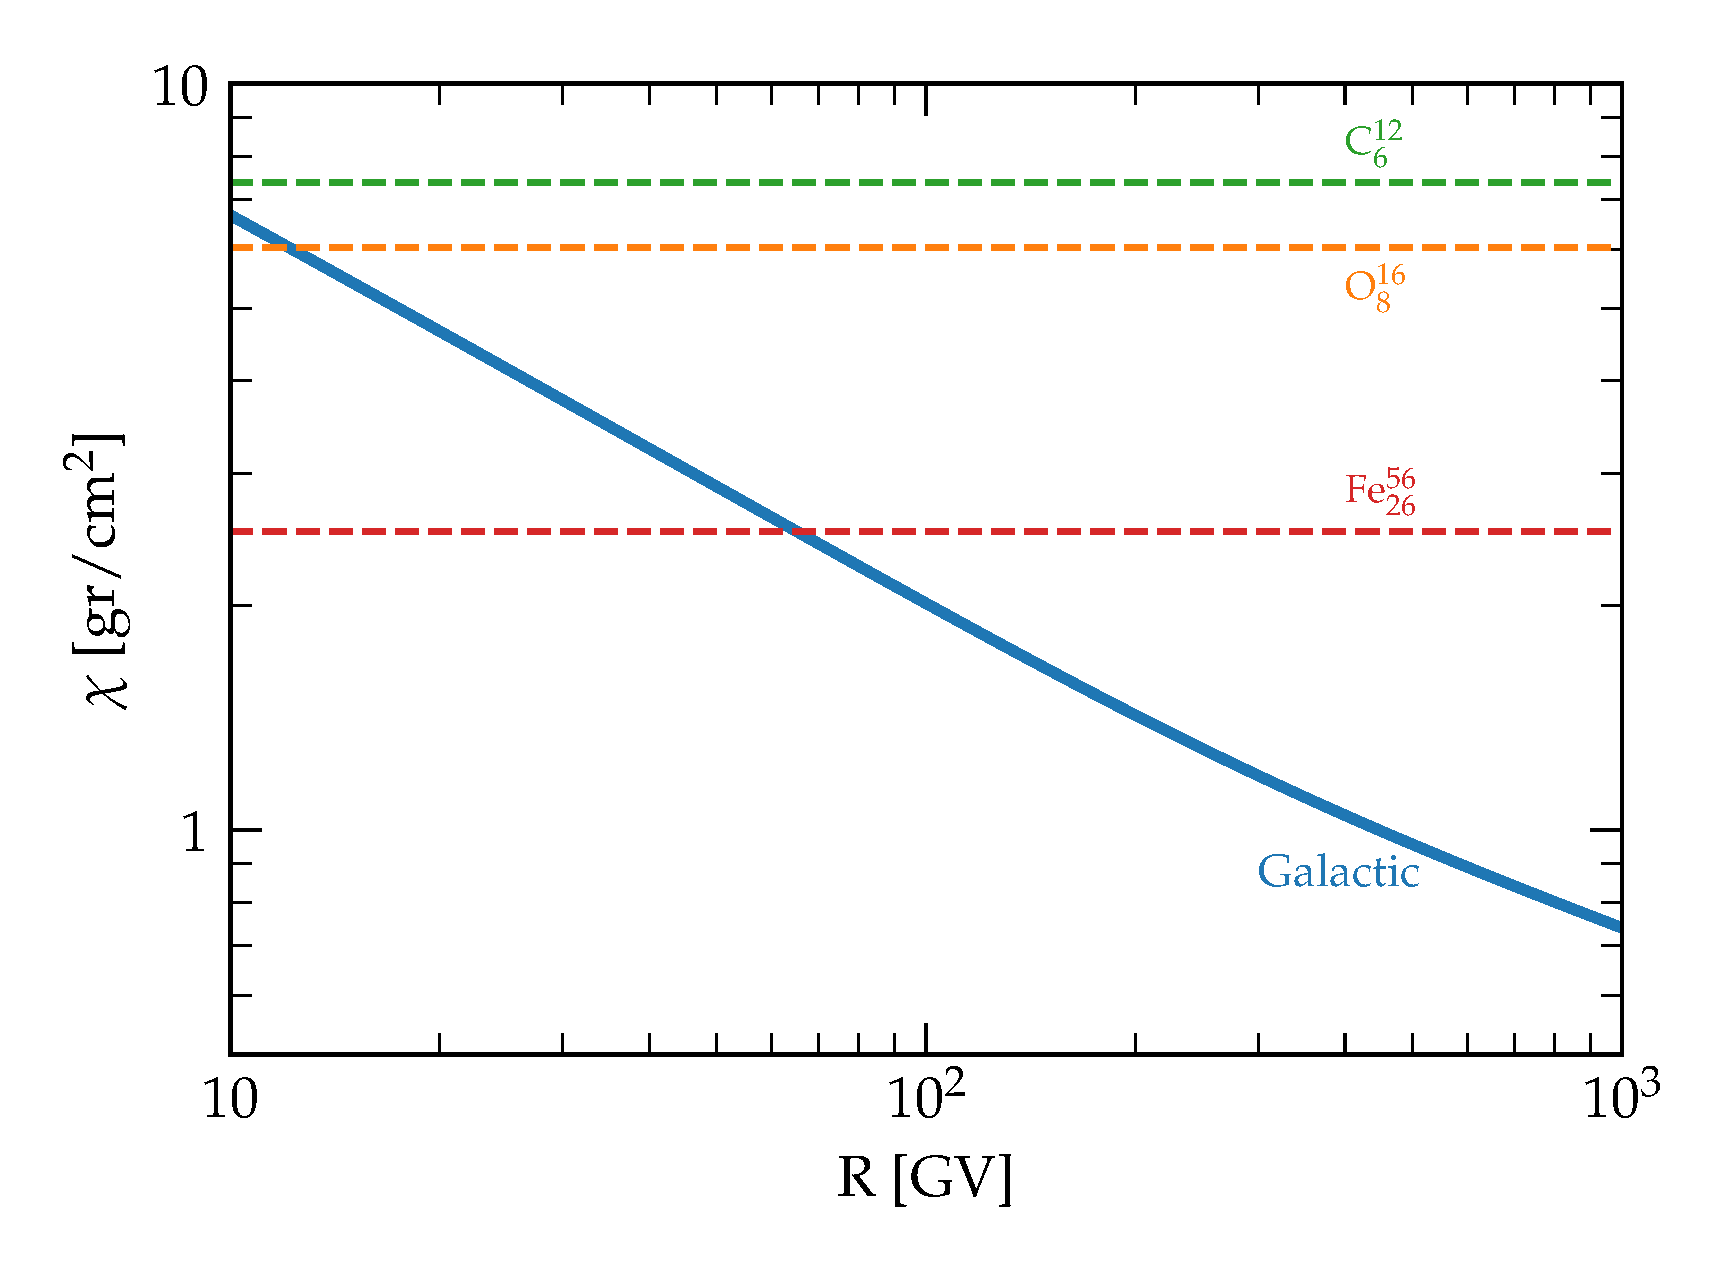
\includegraphics[width=0.6\textwidth]{figures/grammage_critical.pdf}
\caption{The grammage corresponding to the best fit model described in~\cite{Schroer2021prd} as a function of rigidity is shown as a solid blue line. The dashed lines refers to carbon (green), oxygen (orange), and iron (red) inelastic critical grammage.}
\label{fig:grammage}
\end{figure}

%%%%%%%%%% SECTION %%%%%%%%%%
\section{The Secondary-to-Primary Ratio}
\label{sec:secondaryoverprimary}

As mentioned in the Introduction, light and fragile elements such as lithium, beryllium, and boron are mainly synthesized through the collisions of galactic CRs with the interstellar gas in the Galaxy. Here we investigate the production of these elements, and how they constrain CR models for Galactic propagation. 
%
For the sake of simplicity, we focus on a case with only carbon as the primary species ($\alpha^\prime = \text{C}$), whereas boron is almost exclusively created in secondary processes ($\alpha = \text{B}$).

The solution for carbon has been obtained in the previous section and is given by:
%
\begin{equation}
f_{0,\rm C}(p) = \frac{Q_{0,\rm C}}{2n_{\rm d}h m_{\rm p}c} \frac{1}{\frac{1}{\rchi_{\rm C}(p)} + \frac{1}{\rchi_{\rm cr, C}}}
\end{equation}

Since boron is a pure secondary species, the solution of its transport equation takes the same form as the previous equation, with the injection rate proportional to the equilibrium solution for carbon:
%
\begin{equation}
4 \pi Q_{\rm B}(p) p^2 dp = 2 h n_{\rm d} c \sigma_{\rm C \rightarrow B} \delta(z) 4 \pi f_{\rm C}(p^\prime) p^{\prime \, 2} dp^\prime
\end{equation}

Here, $A$ is the atomic number of carbon, and the Jacobian $\frac{dp'}{dp} = \frac{A}{A-1}$ is introduced to ensure conservation of energy per nucleon.

The spectrum of boron in the disc is then given by:
%
\begin{equation}
f_{0,\rm B}(p) 
%= \frac{Q_{0, \rm B}(p)}{2 n_{\rm d} h m_{\rm p} c} \frac{1}{\frac{1}{\rchi_{\rm B}(p)} + \frac{1}{\rchi_{\rm cr, B}}}
= \frac{\sigma_{\rm C \rightarrow B}}{m_{\rm p}}  \frac{1}{\frac{1}{\rchi_{\rm B}(p)} + \frac{1}{\rchi_{\rm cr, B}}} f_{0, \rm C}\left(\frac{A}{A-1}p\right) \left(\frac{A}{A-1} \right)^3~.
\end{equation}

The approximation \( A \gg 1 \) leads to the B/C ratio as:
%
\begin{remark}
\begin{equation}
\frac{\rm B}{\rm C} \simeq \frac{1}{\rchi_{\rm cr, C\rightarrow B}} \left(\frac{1}{\rchi(p)} + \frac{1}{\rchi_{\rm cr, B}}\right)^{-1}
\label{eq:chibc}
\end{equation}
\end{remark}

It is important to note that the boron-to-carbon ratio is independent of the primary source and is solely a function of the grammage and relevant cross-sections.

Once again, it is useful to consider he two limits of strong and weak spallation. 
%
In the case of strong spallation:
%
\begin{equation}
\frac{\rm B}{\rm C} \oset{\rchi \gg \rchi_{\rm cr}}{\, \longrightarrow \,} \frac{\rchi_{\rm cr, B}}{\rchi_{\rm cr, C\rightarrow B}} 
= \frac{\sigma_{\rm C \rightarrow B}}{\sigma_{\rm B}} 
\simeq 0.3
\end{equation}

This results in a constant B/C ratio as a function of energy, with the value determined solely by the cross-sections~\cite{Evoli2019prd}.

In the opposite limit:
%
\begin{equation}
\frac{\rm B}{\rm C} \oset{\rchi \ll \rchi_{\rm cr}}{\, \longrightarrow \,} \frac{\rchi(p)}{\rchi_{\rm cr, C\rightarrow B}} \propto \frac{1}{D(p)}
\label{eq:bchene}
\end{equation}

Hence, in this limit, the B/C ratio is expected to decrease with increasing energy. 
%
Moreover, by measuring the B/C ratio as a function of energy, we can estimate the energy dependence of the grammage and, consequently, of the diffusion coefficient of Galactic CRs.

It is difficult to overemphasize the significance of this result. 
%
The recent AMS-02 data on secondary-to-primary ratios (see figure~\ref{fig:bcams02}) clearly demonstrate that the B/C ratio decreases with increasing rigidity above $\sim$10 GV. %, exhibiting a scaling behavior approximately proportional to the rigidity raised to the power of $\simeq -1/3$. 
%
This indicates that we are operating in the regime of weak spallation, allowing us to infer the Galactic grammage from this observable.
%
A quick fit to data shown in figure~\ref{fig:bcams02}, using $\sigma_{\rm C \rightarrow B} \simeq 60$~mb, indicates that the grammage is of the order of $8.5$~gr cm$^{-2}$ at $\simeq 10$~GV, exhibiting a scaling behavior approximately proportional to the rigidity raised to the power of $\simeq -1/3$. 

Furthermore, by leveraging the observed slope of the proton spectrum, around 2.8 in the energy range 20-200 GeV (see figure~\ref{fig:protonshe}), we can estimate the injection slope $\gamma$ by recovering from~\ref{sec:protons} that $\gamma + \delta \approx 2.8$, guiding us to $\gamma \approx 2.4$. 
%
Consequently, we arrived to the conclusion that the energy spectra of CRs at their sources must be relatively \emph{soft}, challenging the predictions based on the original version of DSA~\cite{Capriolilecturenotes}.

Note that~\ref{eq:grammage} shows that by measuring the grammage, we can only determine the combination $H/D$, and therefore we cannot determine the normalization of the diffusion coefficient without the knowledge of the halo size.

\begin{figure}
\centering
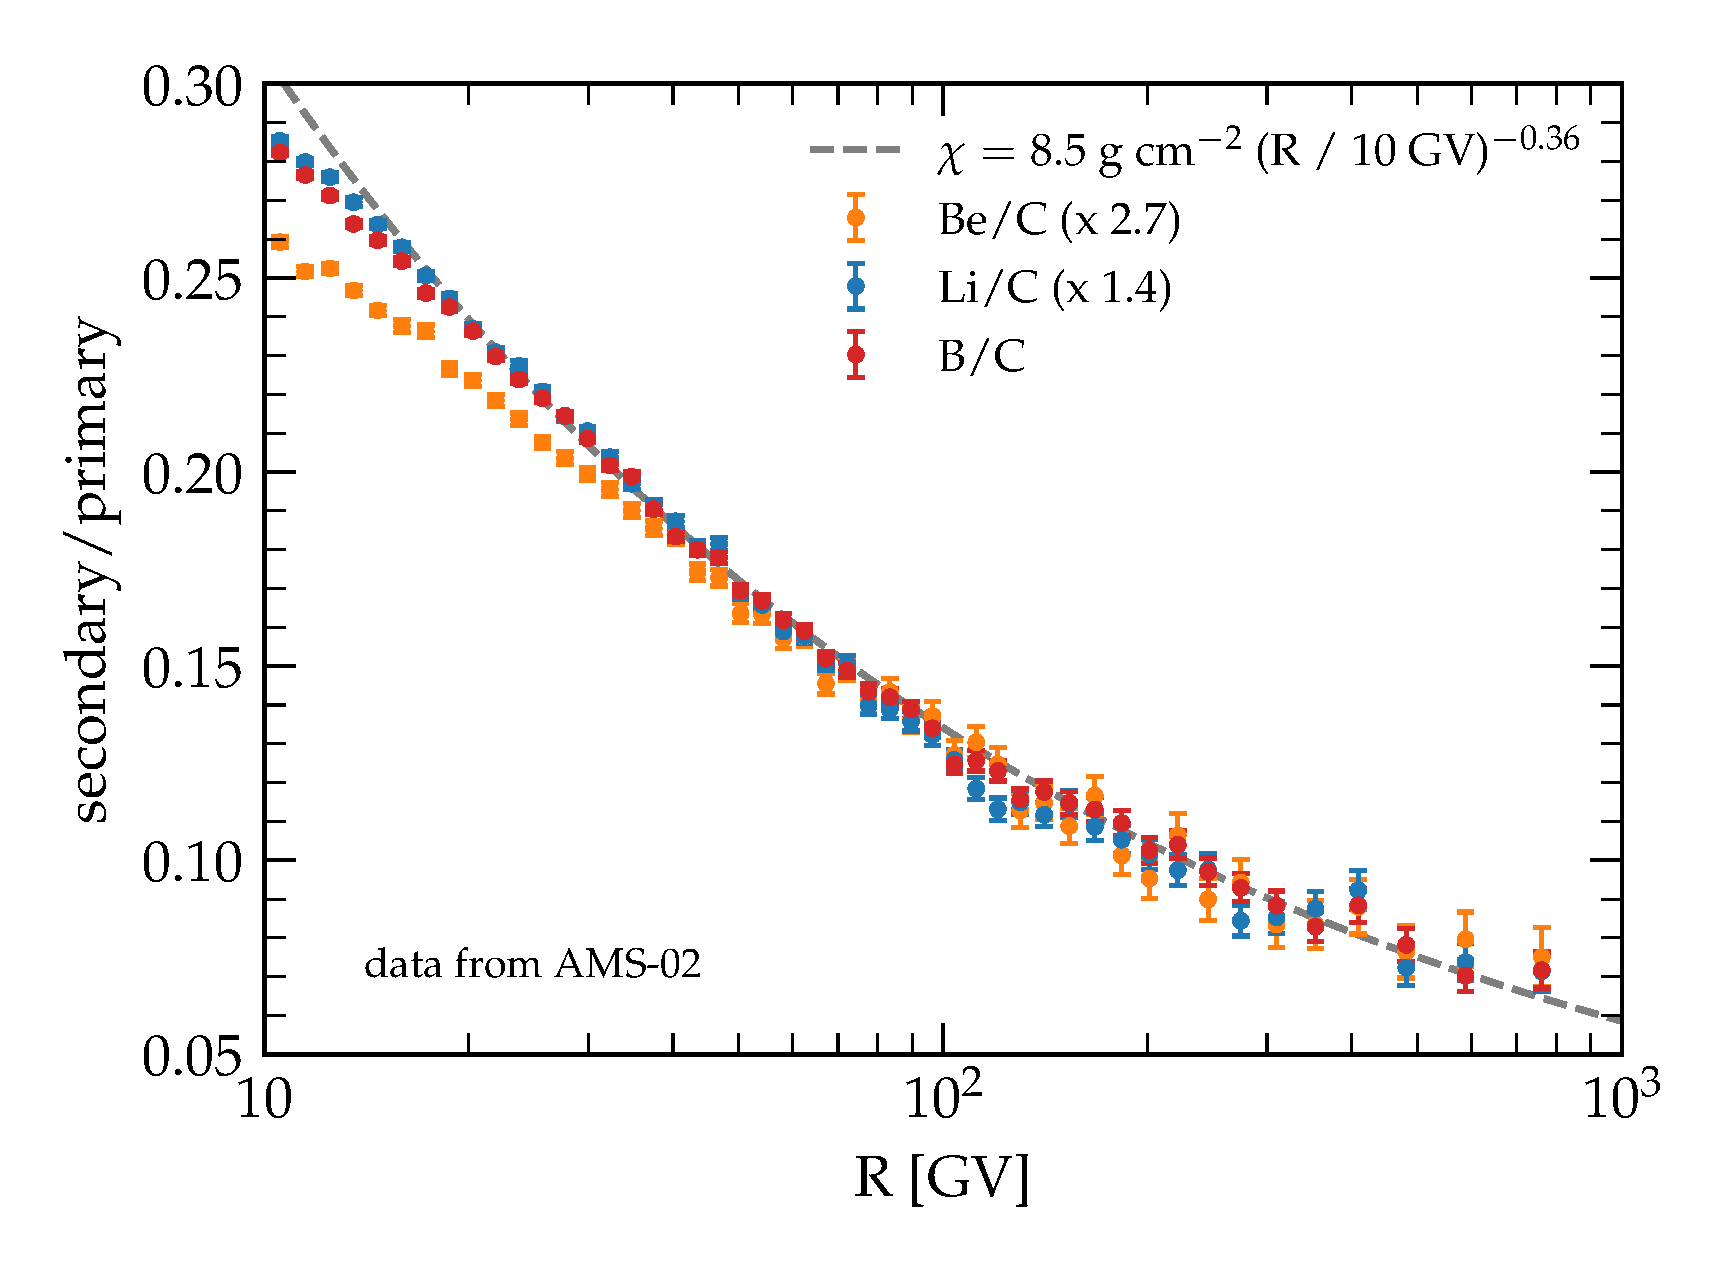
\includegraphics[width=0.6\textwidth]{figures/LiBeB_C_AMS02.pdf}
\caption{Secondary-to-primary ratios as function of rigidity measured by the AMS-02 experiment~\cite{AMS02libeb}. The power-law fit at high energies is also shown.}
\label{fig:bcams02}
\end{figure}

To access the diffusion coefficient, we can make certain assumptions about the size of the Galactic halo. 
%
In the 1960s, it was proposed that observing radio emission from our Galaxy could provide insights into the region where CRs reside~\cite{Ginzburg1961ptps}. This is because radio emission is generated through synchrotron radiation emitted by high-energy electrons. The morphology of the radio emission indicates that it extends well beyond the Galactic disc, where magnetic fields allow particle diffusion to occur.

The region where CRs are predominantly found has a scale of approximately kiloparsecs, significantly larger than the size of the Galactic disc. By utilizing the B/C ratio to estimate $H/D$ and making assumptions about $H$, we can then determine the diffusion coefficient, $D$, and subsequently calculate the average time that CRs spend within the Galaxy, given by $H^2/D$. 

At around 10 GeV, B/C amounts roughly to $\sim 0.3$, which implies\footnote{We have employed equation~\eqref{eq:grammage} in conjunction with the relationship $2h \rho_{\rm d} = \mu_{\rm d}$.} a confinement time of approximately $\sim$100~Myr for $H \sim 3$~kpc, and it decreases as the energy increases.

To delve deeper into this topic, we require a reliable method for measuring this time. In the upcoming section, we will explore how secondary unstable isotopes, which decay with a timescale comparable to the confinement time, can serve as a cosmic clock, enabling us to estimate the Galactic residence time.

Combining this information with the grammage, which yields $H/D$, will allow us to obtain the average value of the diffusion coefficient on Galactic scales.

As we will discuss in~\ref{sec:implications}, these advancements will pave the way for a theoretical comprehension of the microphysics behind the scattering and diffusion of cosmic particles by the fluctuations present in the interstellar turbulent magnetic fields.

\begin{figure}
\centering
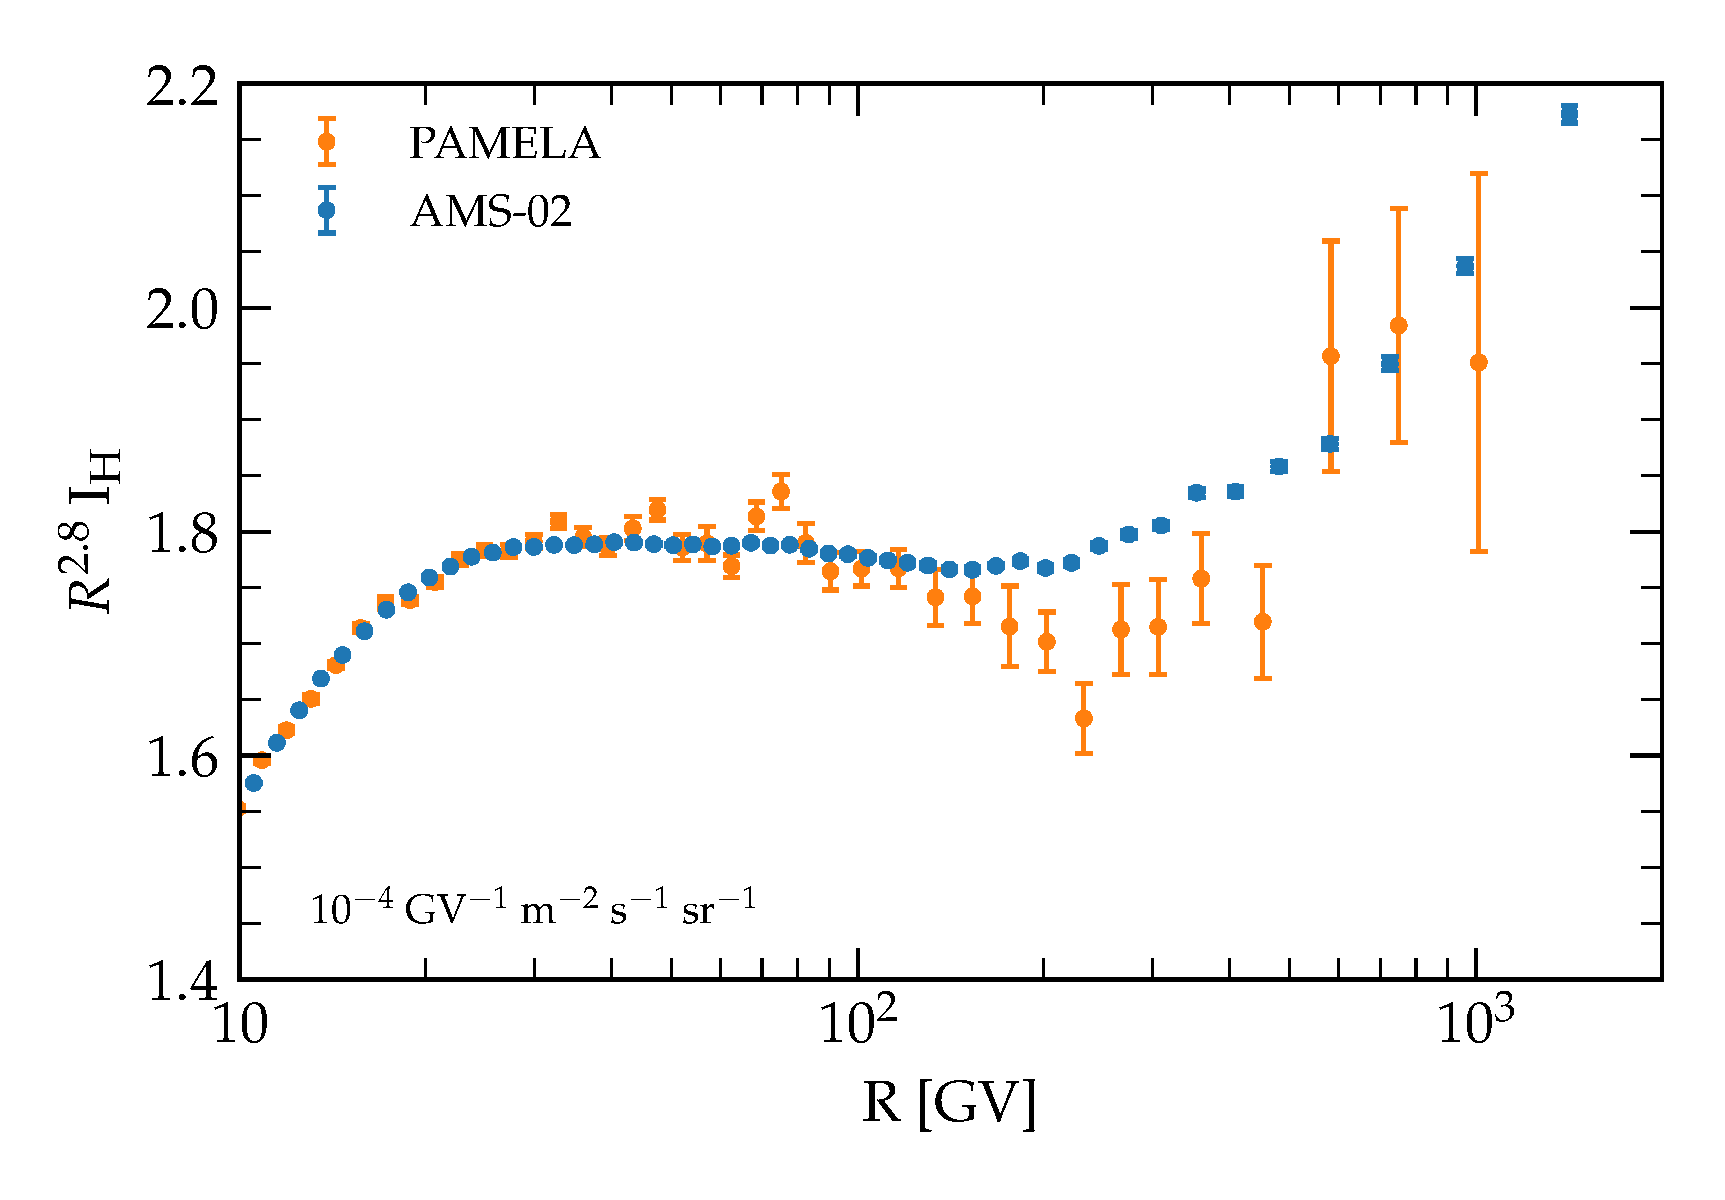
\includegraphics[width=0.6\textwidth]{figures/protons_he.pdf}
\caption{The spectrum of protons as function of rigidity, measured by the AMS-02, and PAMELA experiments~\cite{AMS02results,PAMELA.2011.proton}.}
\label{fig:protonshe}
\end{figure}

The scrupulous reader may have noticed in figure~\ref{fig:protonshe} that the canonical slope, approximately $\sim 2.8$, does not extend up to very high energies. Instead, the CR spectrum exhibits a notable change of slope, commonly referred to as a \emph{break}, at an energy around $400$~GeV, where it hardens to about $\sim 2.6$.
%
At these energies, however, the equilibrium spectrum must be determined by the ratio $Q(p)/D(p)$, where both quantities are assumed to follow a pure power-law behavior. 

Prior to questioning well-established theoretical models to seek the elusive physical mechanism responsible for this bizarreness, it is crucial to ascertain whether the break should be attributed to the numerator or the denominator of~\ref{eq:finalprimary}. 
%
In other words, we need to identify whether the break occurs at the \emph{injection} stage or during the \emph{transport} of CRs in the Galaxy.

Equation~\eqref{eq:bchene} quickly unravels this conundrum! 

Specifically, being dependent only on grammage, the secondary-over-primary ratio is the key parameter to examine. 
%
If the same change of slope is also present in the B/C ratio, then the conclusion must be that it is due to propagation, indicating a break in the diffusion coefficient. On the other hand, if no such change of slope is observed in the B/C ratio, then we must look for the solution at the injection stage.

\begin{figure}
\centering
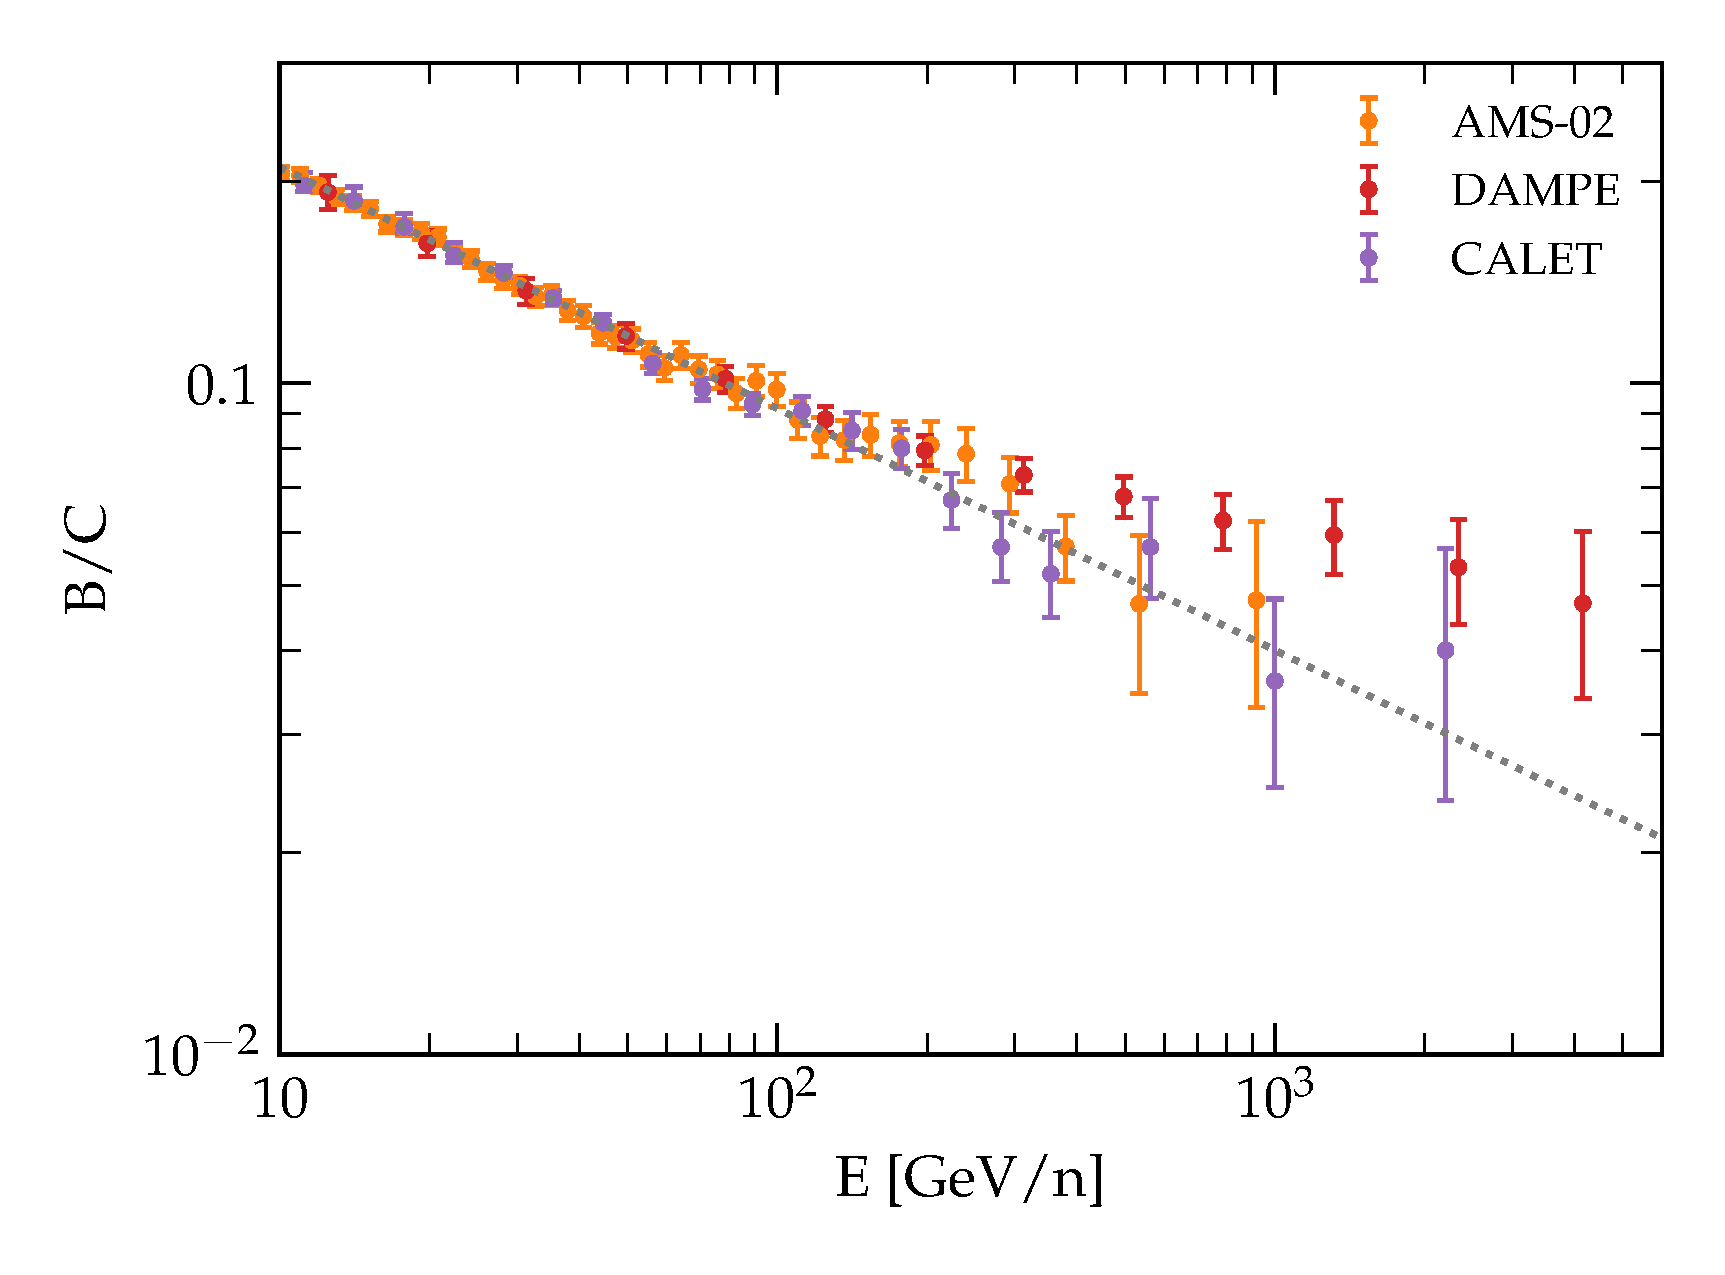
\includegraphics[width=0.6\textwidth]{figures/BC_highenergy.pdf}
\caption{Boron-to-carbon ratio as function of kinetic energy per nucleon measured by the AMS-02~\cite{AMS02results}, CALET~\cite{CALET.2022.BC} and DAMPE~\cite{DAMPE.2022.BC} experiments.}
\label{fig:bchighen}
\end{figure}

As shown in~\ref{fig:bchighen}, where we extend B/C data over the multi-TeV range thanks to measurements by DAMPE and CALET, the situation indeed aligns with the former scenario, and thereby all the current explanations of this feature are given in terms of some alteration in the galactic transport. 
%
These revisions in the transport of CRs might be associated with a spatial dependence of the diffusion coefficient, as proposed in ~\cite{Tomassetti2012apj}, or due to the transition from selfgenerated turbulence to preexisting turbulence, see, e.g.,~\cite{Evoli2018prl}.

At such, the recently reported departures from an otherwise uninteresting scale-free power-law behavior in the galactic CR spectra are of paramount importance, as they offer valuable insights into the fundamental mechanisms governing the propagation of CRs in magnetized environments.

%%%%%%%%%% SECTION %%%%%%%%%%
\section{Unstable nuclei: the case of beryllium}
\label{sec:unstable}

The average time that CRs spend in the Galaxy before escaping can be determined by studying the suppression of the flux of unstable nuclei due to radioactive decay. By comparing the fluxes of two isotopes of the same chemical element—one stable and the other unstable—it is possible to measure this suppression and estimate $\tau_{\rm esc}$.

Beryllium is an element that is very rare in ordinary matter, and the majority of beryllium nuclei in CRs are secondary particles formed through the fragmentation of heavier nuclei. 
%
It has two stable isotopes, $^9$Be and $^7$Be (if fully ionized), as well as one $\beta^-$ unstable isotope, $^{10}$Be, with a half-life of $\tau_{1/2} = (1.386 \pm 0.016)$ Myr~\cite{Chmeleff2010nimb}. 
%
The decay of $^{10}$Be mainly produces $^{10}$B, thus altering the abundance of this stable element.

The transport equation for $^{10}$Be can be treated as that of a secondary species, assuming (for simplicity) only one parent nucleus. 
%
Additionally, a term describing decay in the Galaxy reference frame is included:
%
\begin{equation}
-\frac{\partial}{\partial z} \left[ D_{\rm Be} \frac{\partial f_{\rm Be}}{\partial z} \right] =
- \frac{f_{\rm Be}}{\tau_{\rm f, Be}} 
- \frac{f_{\rm Be}}{\gamma \tau_{\rm d, Be}} 
+ \frac{f_{\rm C}}{\tau_{\rm f, C \rightarrow Be}} 
\end{equation}
%
Here, $\tau_{\rm d} = \tau_{1/2} / \ln(2)$ represents the rest-frame lifetime of $^{10}$Be, and $\gamma$ accounts for time dilation effects.
%
At sufficiently high energies, $^{10}$Be decays on a timescale longer than $\tau_{\rm esc}$, effectively behaving as a stable isotope.

It is worth emphasizing that this is the first case we have discussed where the source or loss term in the transport equation does not exhibit a $\delta$-function shape in $z$. This distinction arises due to the inclusion of the decay term, which introduces a new complexity that necessitates a dedicated approach for solving the corresponding transport equation.

Outside the disk $z \neq 0$, the transport equation becomes:
%
\begin{equation}
-\frac{\partial}{\partial z} \left[ D_{\rm Be} \frac{\partial f_{\rm Be}(z)}{\partial z} \right] + \frac{f_{\rm Be}(z)}{\gamma\tau_{\rm d, Be}} = 0
\end{equation}

Unlike the case of stable elements, the diffusive flux is not conserved. 
%
To find a solution, we assume the form:
%
\begin{equation}
f(z) = A {\rm e}^{-\alpha z} + B {\rm e}^{\alpha z}
\end{equation}
%
which implies $\alpha^{-1} = \sqrt{D \gamma\tau_{\rm d}}$, where we have assumed that the diffusion coefficient is spatially constant.

By imposing the appropriate boundary conditions, we obtain (introducing $y \equiv {\rm e}^{\alpha H}$):
%
\begin{equation}
\frac{f_{\rm Be}(z)}{f_{\rm Be,0}} =  -\frac{y^2}{1 - y^2} {\rm e}^{-\alpha z} + \frac{1}{1- y^2} {\rm e}^{\alpha z} 
\label{eq:bespatial}
\end{equation}

The value of the distribution function at $z=0$ can be obtained by integrating above and below the disk:
%
\begin{equation}
\left. -2 D_{\rm Be} \frac{\partial f_{\rm Be}(T)}{\partial z} \right|_{0^+} =
- 2 h n_{\rm d} c \sigma_{\rm Be} f_{0, \rm Be}
+ 2 h n_{\rm d} c \sigma_{\rm C \rightarrow Be} f_{0, \rm C} 
\end{equation}

To obtain the flux, we utilize equation~\eqref{eq:bespatial}, yielding:
%
\begin{equation}
\left. \frac{\partial f_{\rm Be}(T)}{\partial z} \right|_{0^+} = \alpha \frac{1+y^2}{1-y^2} \, f_{\rm Be,0}
\end{equation}

Combining these equations, we arrive at:
%
\begin{equation}
f_{\rm Be,0}(p) \left[  \frac{\sigma_{\rm Be}}{m_{\rm p}} - \frac{1}{c m_{\rm p} h n_{\rm d}} \sqrt{\frac{D_{\rm Be}(p)}{\gamma \tau_{\rm d, Be}}} \frac{1+y^2}{1-y^2} \right] = 
\frac{\sigma_{\rm C\rightarrow Be}}{m_{\rm p}} f_{\rm C,0}(p)
\end{equation}

Alternatively, one can write it in terms of grammages
%
\begin{equation}
\frac{f_{\rm Be,0}}{f_{\rm C,0}}(p) = 
\frac{1}{\rchi_{\rm cr, C \rightarrow Be}}  \left[  \frac{1}{\rchi_{\rm cr, Be}} + \frac{1}{\rchi_{\rm Be}^\prime(p)} \right]^{-1}  
\end{equation}
%
where $\rchi^\prime$ represents the grammage modified by the decay term and can be expressed as:
%
\begin{equation}
\rchi^\prime_{\rm Be}(p) = \rchi_{\rm Be}(p) \frac{1}{\alpha H} \frac{y^2 - 1}{y^2 + 1} 
\end{equation}

We observe that at high energies, when the proper decay time becomes much larger than the confinement time ($\gamma \tau_{\rm d} \gg \frac{H^2}{D}$), we have $\alpha H \rightarrow 0$ and expanding in Taylor series:
%
\begin{equation} 
\rchi_{\rm Be}^\prime(p) 
\oset{\gamma\tau_{\rm d} \gg \tau_{\rm esc}}{\longrightarrow} 
\rchi_{\rm Be}(p)
\end{equation}

\begin{figure}
\centering
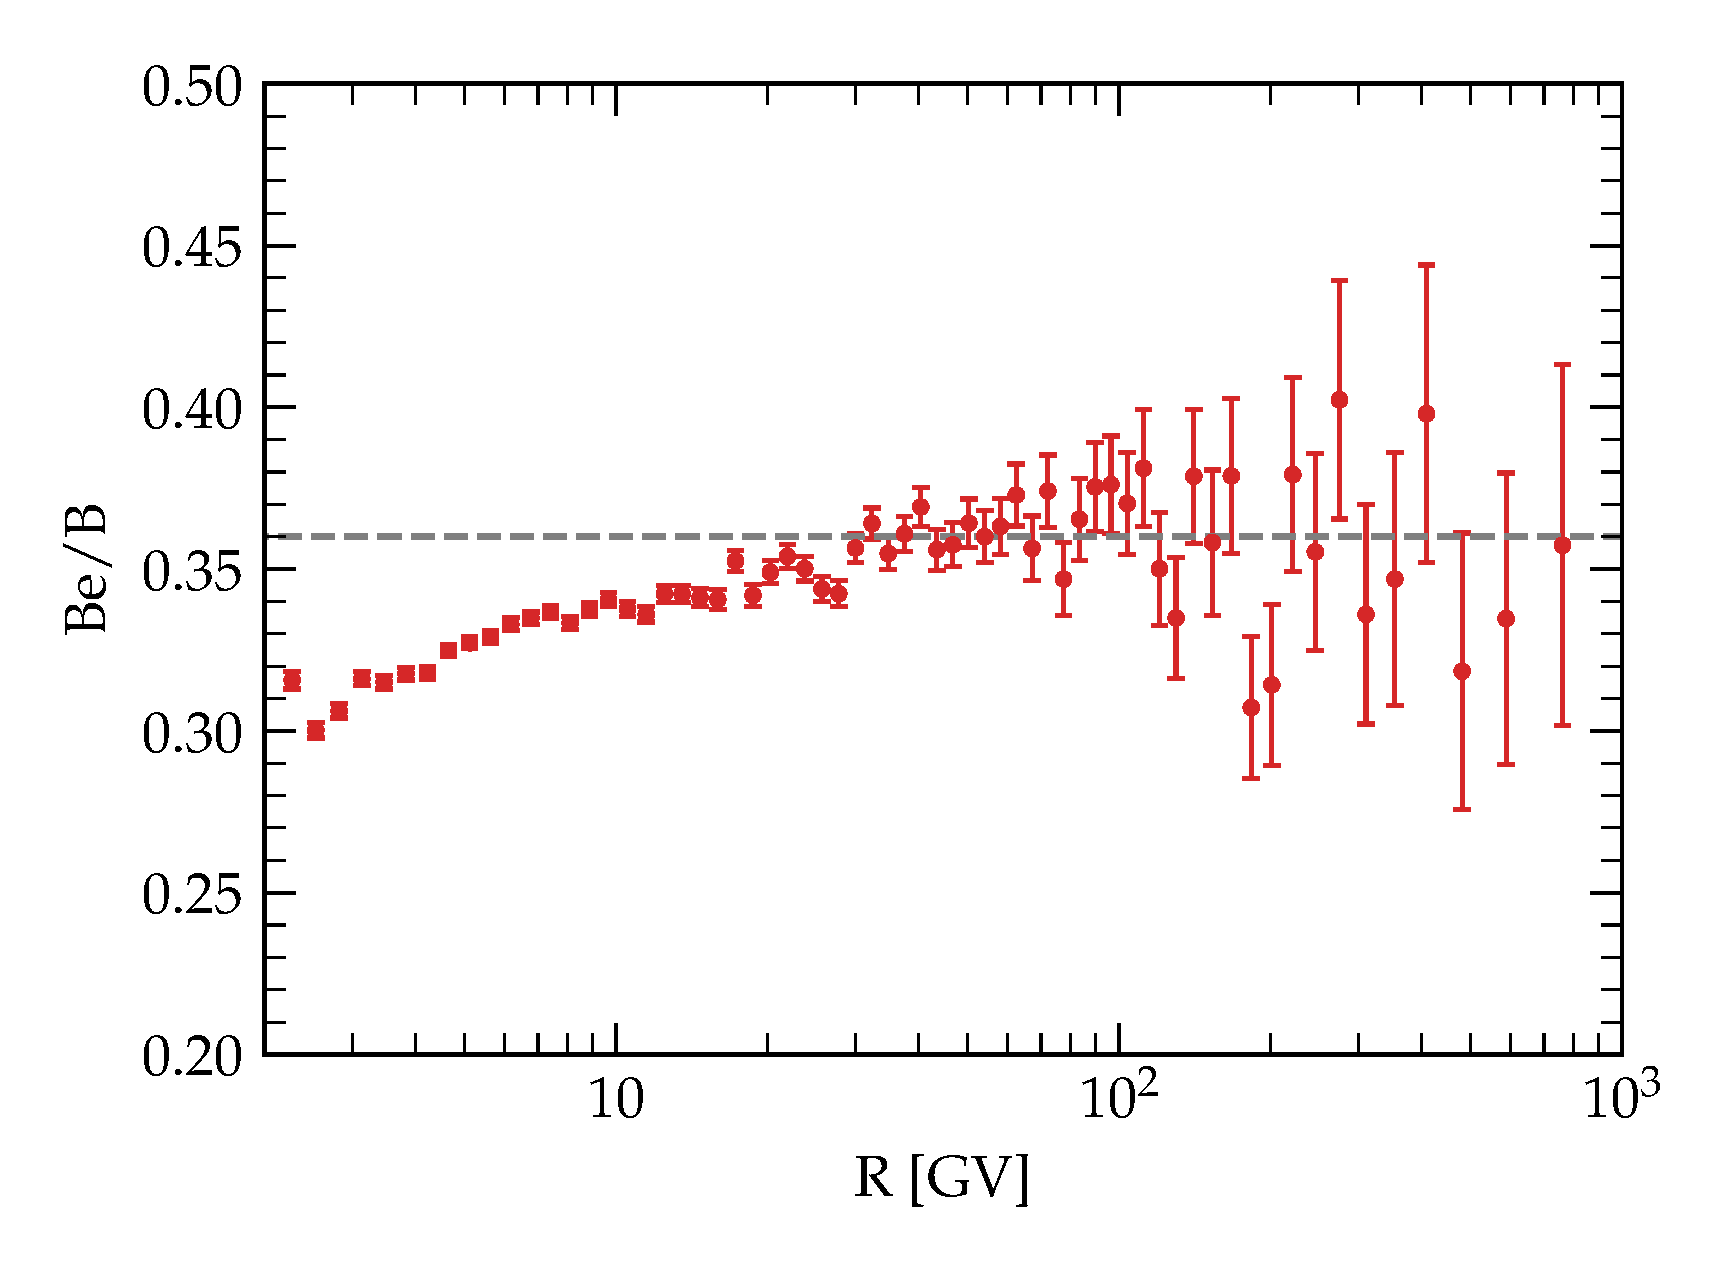
\includegraphics[width=0.6\textwidth]{figures/BeB_AMS02.pdf}
\caption{Ratio of Beryllium over Boron fluxes as measured by AMS-02~\cite{AMS02libeb}. The dotted line shows the case without decay for 10Be.}
\label{fig:beb}
\end{figure}

As expected $\tau_{\rm d}$ cancels out from the grammage, and we recover in this limit the solution obtained for a stable element.

In the opposite limit, $y \rightarrow \infty$, and the modified grammage $\rchi_{\rm Be}^\prime(p)$ approaches a simplified form:
%
\begin{equation}
\rchi_{\rm Be}^\prime(p) 
\oset{\gamma\tau_{\rm d} \ll \tau_{\rm esc}}{\longrightarrow} 
m_{\rm p} n_{\rm d} h c \sqrt{\frac{\gamma\tau_{\rm d, Be}}{D_{\rm Be}(p)}} = 
m_{\rm p} \bar n c \sqrt{\gamma \tau_{\rm d} \tau_{\rm esc}} 
\label{eq:be10be9}
\end{equation}

It is important to note that in this case, it becomes crucial to account for the additional contribution to boron production arising from the decay of beryllium. This contribution can be analytically calculated using the distribution of parent beryllium in the halo, as outlined in equation~\eqref{eq:bespatial} (a detailed derivation of this contribution is provided in~\cite{Evoli2020prd}).

In the given context, the ratio of $^{10}$Be to $^9$Be fluxes can be approximated using equation~\eqref{eq:be10be9}, which relates it to the grammage ratio:
%
\begin{equation}
\frac{\rm {^{10}}Be}{\rm {^{9}}Be} \simeq \frac{\rchi^\prime_{\rm Be}}{\rchi_{\rm Be}} = \sqrt{\frac{\gamma \tau_d}{\tau_{\rm esc}}}
\label{eq:chibe10be9}
\end{equation}

The preliminary results from the AMS-02 experiment indicate a value of $\frac{\rm {^{10}}Be}{\rm {^{9}}Be} \sim 0.3$ at a kinetic energy per nucleon $T \sim 10$ GeV/n. Inverting the equation, we can estimate the escape time as $\tau_{\rm esc} \simeq 200$~Myr.

Furthermore, the relationship between the scale height $H$ and the escape time $\tau_{\rm esc}$ can be quantitatively expressed as:
%
\begin{equation}
H \sim 7 \, \text{kpc} \left(\frac{\tau_{\rm esc}}{200 \, \text{Myr}}\right) \left(\frac{\rchi}{10 \, \text{g cm}^2}\right)^{-1}
\end{equation}
%
roughly confirming the scaling estimated with the synchrotron emission.

While directly measuring the CR confinement time $\tau$ by comparing the flux of $^{10}$Be to that of $^9$Be remains challenging due to the difficulty of separating in mass the two isotopes, the AMS-02 experiment provides access to the total flux of beryllium, encompassing $^7$Be, $^9$Be, and $^{10}$Be, as well as the total flux of boron.
%
Examining the ratio of Be/B still allows us to obtain valuable information, considering that this ratio is influenced by the decay of $^{10}$Be, affecting both the numerator and the denominator (see figure~\ref{fig:beb}).

The observed behavior of the Be/B ratio at rigidities $\lesssim 30$ GV, where the ratio changes due to the decay of $^{10}$Be and not solely based on the production cross-section ratio, suggests that the escape timescale is not significantly faster than the decay timescale at that energy.

A dedicated analysis of this process, as reported in~\cite{Evoli2020prd,Weinrich2020aab,Maurin2022aa}, indicates that $H$ is approximately 6 kpc, although the possibility of a larger value cannot be excluded.

%%%%%%%%%% SECTION %%%%%%%%%%
\section{Electrons and positrons}
\label{sec:leptons}

The fraction of leptons (electrons + positrons) in the total CR flux may be small, but their unique properties make them crucial for studying fundamental astrophysical problems, such as CR propagation and the search for sources of antimatter in the Universe.

Theoretical considerations suggest that CR electrons consist of a primary component, accelerated possibly by SuperNova Remnants (SNRs) along with nuclei, and a secondary component originating from inelastic collisions between CR nuclei (mostly protons and helium) and the ISM. However, this secondary contribution accounts for only a small fraction (less than 4\%) of the total electron flux~\cite{Moskalenko1998apj,Delahaye2010aa,Evoli2021prd}.

In the standard model of CR origin, positrons were considered to be predominantly of secondary production, with a spectrum steeper than that of both primary protons and secondary nuclei (like boron) due to radiative losses. Within this framework, the positron fraction, defined as the ratio of positron flux to the sum of electrons and positrons, was expected to decrease with increasing energy. Early measurements of the positron fraction provided preliminary and intriguing evidence for a flat or even increasing trend, contradicting the standard CR transport scenario. However, the statistical limitations of these early measurements, attributed to the very low positron flux in cosmic radiation, prevented robust conclusions. Nonetheless, this finding received strong confirmation from the PAMELA experiment, which demonstrated a growing positron fraction with energy, at least up to approximately 100 GeV~\cite{PAMELA.2009.posfraction}. The excess was also observed by Fermi-LAT, which utilized Earth's magnetic field to distinguish between electrons and positrons~\cite{FERMI.2012.posfraction}. 
%
Subsequently, the positron excess was further confirmed and measured with higher accuracy at even higher energies by the AMS-02 experiment aboard the International Space Station. Thanks to its extended energy range, the AMS-02 experiment reported the first experimental observation of the positron fraction reaching a maximum around $\sim$500 GeV, followed by a sharp drop at higher energies~\cite{AMS02.2013.posfraction}.

In addition, the unambiguous measurement of electron and positron spectra separately revealed that the rise in the positron fraction is due to an excess of positrons rather than a deficit of electrons~\cite{AMS02.2019.electrons}.

These discoveries have unveiled a new population of sources that are primarily responsible for the production of electron-positron pairs. Among the various possibilities, galactic pulsars emerge as the most likely candidates for these leptonic sources, representing a remarkable breakthrough in our comprehension of the acceleration mechanisms occurring in these objects~\cite{Harding1987icrc,Aharonian1995aa,Grasso2009aph,Hooper2009jcap,Delahaye2010aa,Manconi2020prd,Amato2020arxiv}.

The propagation of electrons in the Galaxy is different from that of nuclei. At high energies, radiative losses become a dominant process, as loss-time scales proportionally to $E^{-1}$. Consequently, high-energy electrons have limited lifetimes and can only propagate within a restricted distance range.

For these high-energy electrons, the primary energy loss mechanisms are synchrotron radiation resulting from interactions with interstellar magnetic fields and inverse Compton scattering (ICS) with Galactic radiation fields (such as the cosmic microwave background, infrared, optical, and UV photons).

In the Thompson approximation, neglecting Klein-Nishina corrections to the $\gamma$-e$^-$ cross-section\footnote{In the context of the Galaxy, this assumption encounters some limitations, particularly concerning the ICS of electrons with optical and UV photons. A more accurate approach to ICS reveals spectral features arising from the diminishing Klein-Nishina cross-section of electrons as their energy surpasses around $\sim 40$~GeV when interacting with UV photons~\cite{Agaronyan1985ap,vanderwalt1991mnras,Evoli2020prl}.}, the rate of energy loss can be expressed as follows (see P.D.~Serpico's lecture notes in this volume):
%
\begin{equation}
\left| \frac{dE}{dt} \right| = \frac{4}{3} \sigma_{\rm T} c \gamma^2 \beta^2 (\mathcal U_\gamma + \mathcal U_{\rm B}) = b_0 \left( \frac{E}{10~\rm GeV} \right)^2
\end{equation}
%
Here, $\sigma_{\rm T}$ represents the Thomson cross section, $\mathcal U_\gamma$ denotes the energy density in background photons, and $\mathcal U_{\rm B} = \frac{B^2}{8\pi}$ represents the magnetic field energy density.

In Galactic environments, the energy densities $\mathcal U_i$ typically range from $\mathcal O(0.1-1~\text{eV/cm}^3)$, leading to a value of $b_0$:
%
\begin{equation}
b_0 \sim  10^{-14} \left(\frac{\mathcal U_\gamma + \mathcal U_{\rm B}}{\rm eV/cm^3}\right) \left(\frac{E}{10~\rm GeV}\right)^2 \, \text{GeV} \, \text{s}^{-1}
\end{equation}

The energy loss time turns out to be a \emph{decreasing} function with energy:
%
\begin{equation}
\tau_{\rm loss} \simeq \frac{E}{-dE/dt} \sim 30 \, \text{Myr} \left(\frac{E}{10~\rm GeV}\right)^{-1}
\end{equation}

\begin{figure}[t]
\centering
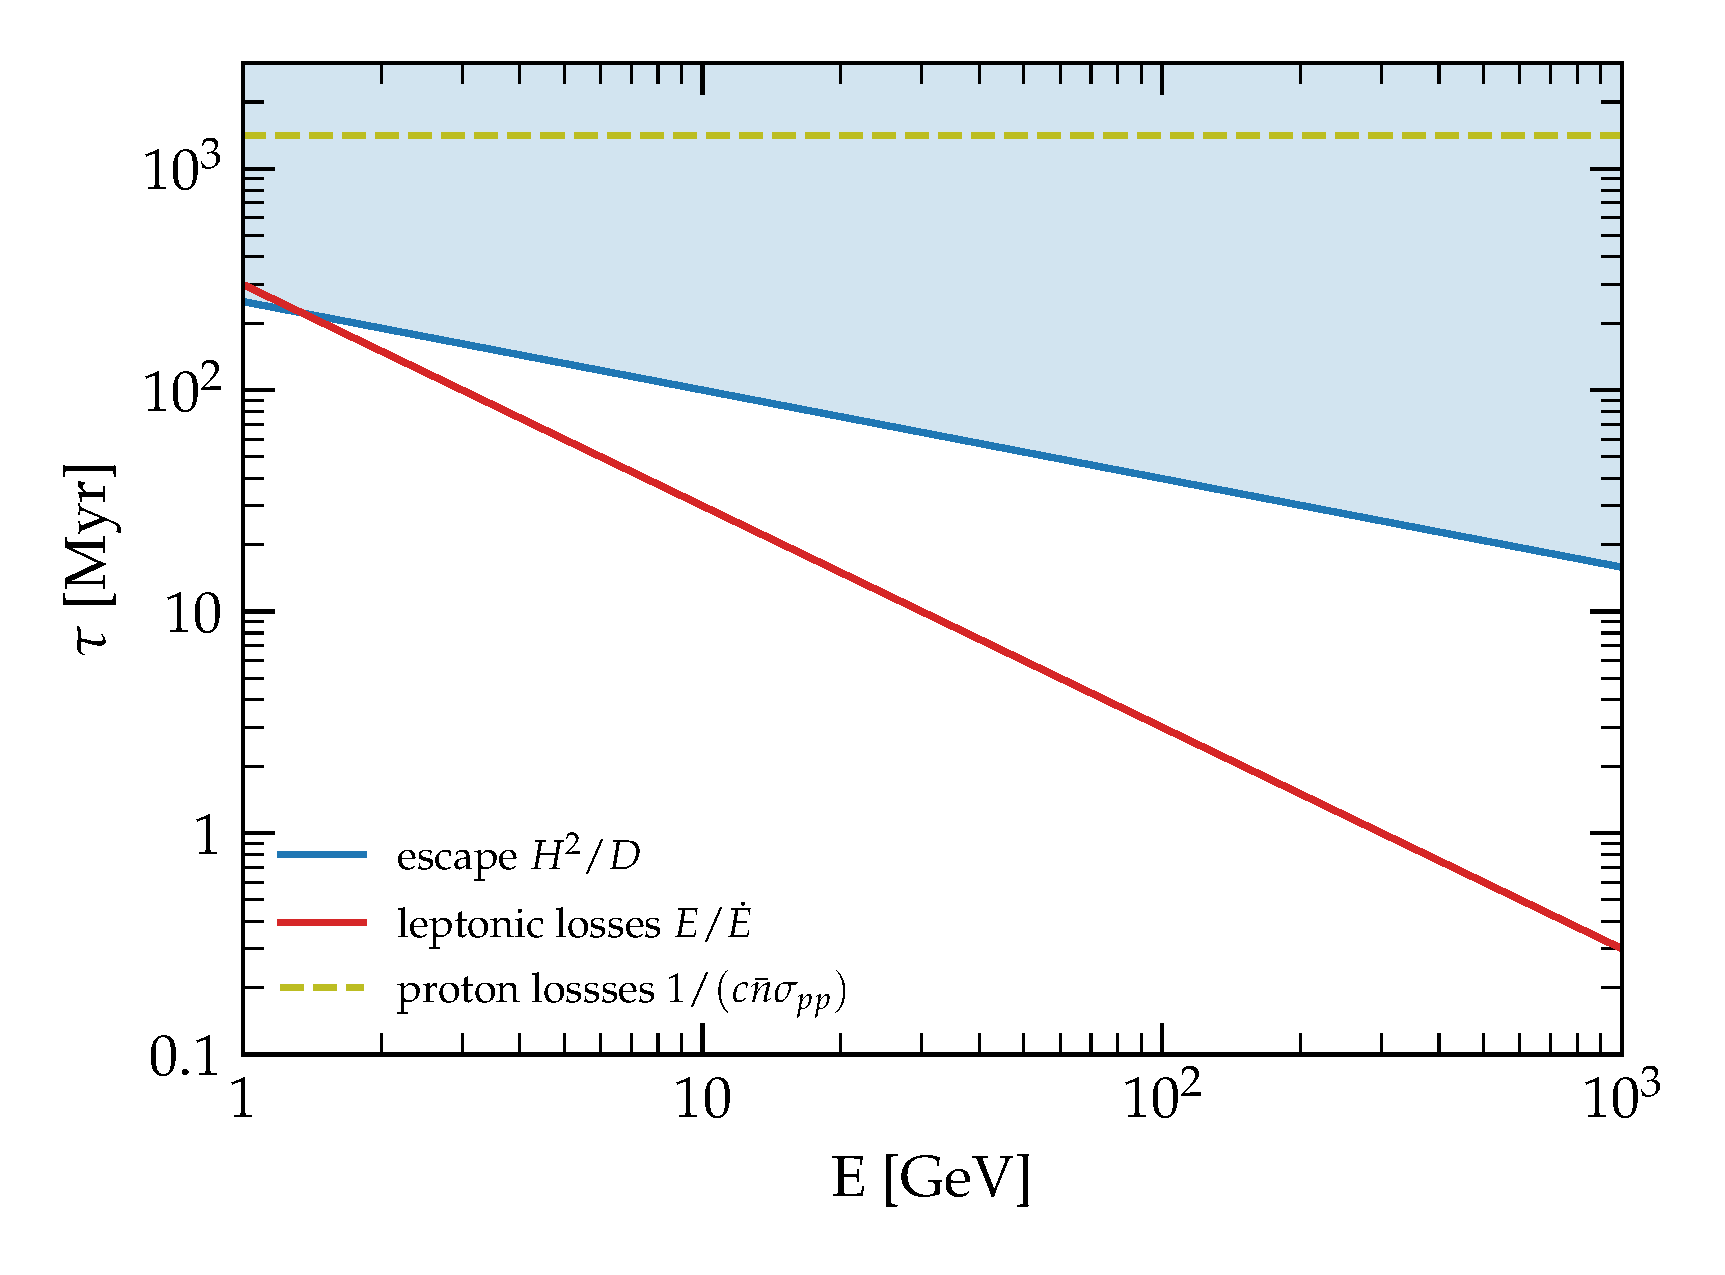
\includegraphics[width=0.6\textwidth]{figures/electron_losses.pdf}
\caption{The escape timescale derived in \S\ref{sec:protons} is confronted with energy loss timescales for protons (inelastic scattering) and leptons (synchrotron + IC) in the Milky Way.}
\label{fig:electronlosses}
\end{figure}

Figure~\ref{fig:electronlosses} provides a comparison between the energy loss timescale for electrons and the CR escape timescale as derived from nuclei. For typical values of CR transport in the ISM, the transition between the two regimes occurs at a few GeV. This implies that the Galaxy acts as an effective calorimeter for leptons, as they are expected to lose a significant portion of their energy during the typical escape time.

The transport equation for leptons is described by\footnote{For CR electrons $p \simeq E$}:
%
\begin{equation}
-\frac{\partial}{\partial z} \left [D \frac{\partial f_e}{\partial z} \right] 
= Q_e(E) \delta(z)
- \frac{1}{E^2} \frac{\partial}{\partial E} \left[ \dot E E^2 f_e \right] 
\end{equation}
%
where $\dot E$ represents the energy loss rate.

To simplify the loss term, it is convenient to approximate it as a catastrophic loss term~\footnote{Notice that assuming $\dot E \propto E^2$ and $f_e \propto E^{-\alpha}$ the relative difference between the two terms is $\sim\alpha$.}:
%
\begin{equation}
-\frac{\partial}{\partial z} \left [D \frac{\partial f_e(E)}{\partial z} \right] = Q_e(E) \delta(z) - \frac{f_e(E)}{\tau_{\rm loss}(E)}  
\label{eq:leptonprop}
\end{equation}
%
allowing the equation to be solved similarly to unstable nuclei, as the energy losses are effective throughout the propagation volume.

In the limit of negligible losses, the solution of equation~\eqref{eq:leptonprop} corresponds to that of a stable species. On the other hand, when losses dominate transport ($\tau_{\rm loss} \ll \tau_{\rm esc}$), the solution can be expressed as:
%
\begin{equation}f_{e,0}(E) 
= \frac{Q_{e,0}(E) \mathcal R_{\rm SN}}{2 \pi R_{\rm d}^2} \frac{\tau_{\rm loss}(E)}{\sqrt{D(E)\tau_{\rm loss}(E)}}
\propto E^{{-\gamma}-\frac{1 + \delta}{2}}
\label{eq:leptonsolution}
\end{equation}

\begin{figure}[t]
\centering
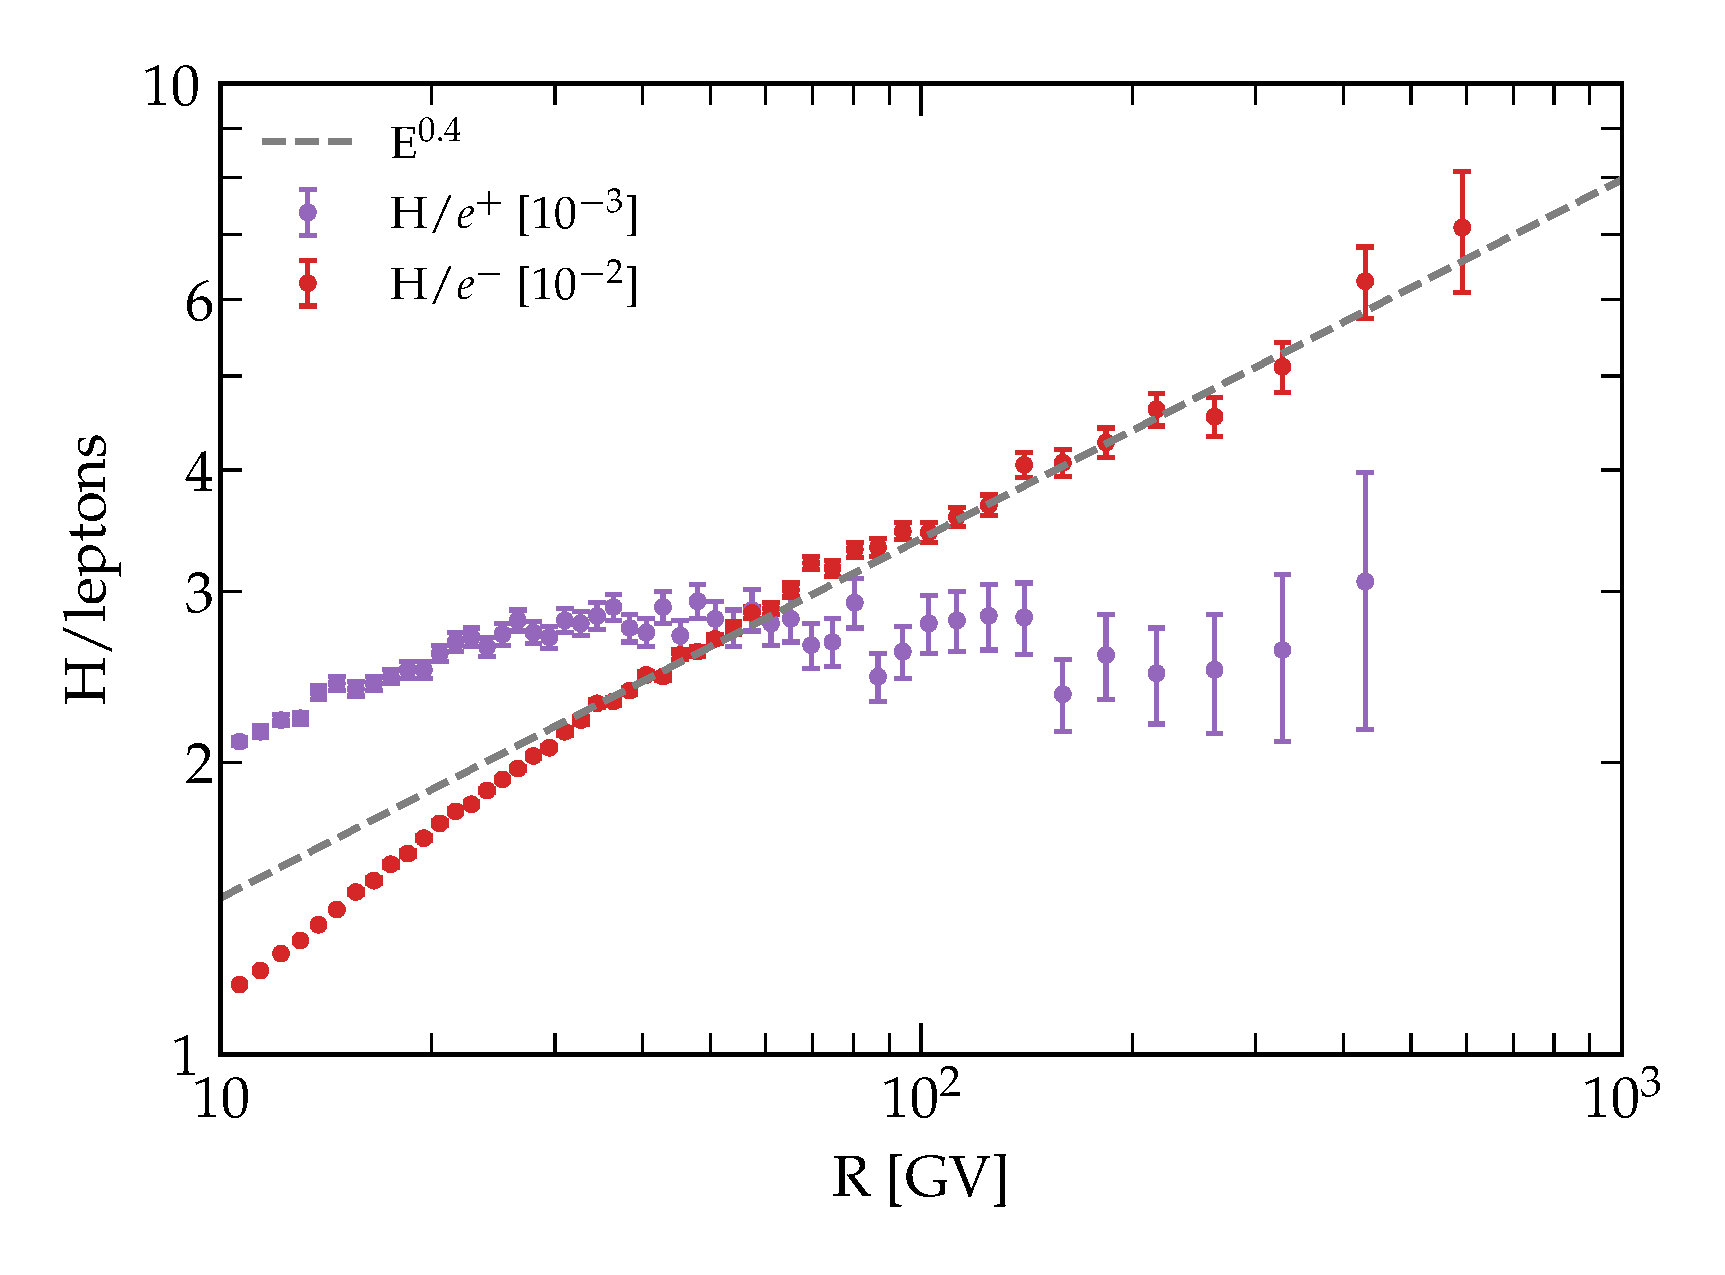
\includegraphics[width=0.6\textwidth]{figures/H_electron_ratio.pdf}
\caption{The electron(positron)-over-proton ratio as measured by AMS-02~\cite{AMS02.2019.electrons}. The high-energy power law fit is also shown as a dashed line.}
\label{fig:protonelectron}
\end{figure}

Thereby, the transition from a diffusion-dominated regime to a losses-dominated regime results in a \emph{softening} of the electron spectrum. This transition leads to a change in slope of
%
\begin{equation}
\Delta \alpha = (-\gamma-\delta) - (-\gamma-\frac{1 + \delta}{2}) = \frac{1 -\delta}{2} \simeq 0.3
\end{equation}

In Galactic CRs, the spectral break is not easily discernible due to the strong influence of solar modulation in the energy range where the break is expected to occur. 
%
Moreover, above the energy range where solar modulation plays a significant role, the most prominent feature in the electron spectrum is the spectral steepening at energies $E \lesssim$ TeV. The spectral break in the electron spectrum is well-described by a broken power-law with a change of slope of approximately $\sim$1~\cite{HESS.2008.leptons,DAMPE.2017.leptons,CALET.2018.leptons}, which is too large to be attributed to the \emph{cooling} break resulting from the transition between the diffusion-dominated and losses-dominated regimes\footnote{However, refer to~\cite{Cowsik1979apj,Lipari2017prd} for instances where unconventional approaches are explored, continuing to challenge the foundational principles outlined in these lecture notes.}. 
%
This further strengthens the evidence that electron transport is predominantly governed by energy losses throughout the entire energy range.

When comparing the proton and electron spectra, see figure~\ref{fig:protonelectron}, the difference in normalization is likely caused by the different injection mechanisms into the acceleration process for electrons and protons, as suggested by previous studies~\cite{Morlino2021mnras}.

On the other hand, we may be tempted to attribute the steeper slope of the electron spectrum solely to their energy losses.
%
Between 50 and 500 GeV, the ratio of proton flux to electron flux is well described by a power law with a slope of $\sim$0.4.

According to the prediction of the diffusion-losses model, this ratio can be expressed as:
%
\begin{equation}
\frac{f_p}{f_e} \propto \frac{E^{-\gamma_p-\delta}}{E^{{-\gamma_e}-\frac{1 + \delta}{2}}} \propto E^{-(\gamma_p-\gamma_e)} E^{\frac{1-\delta}{2}}
\end{equation}
%
where we differentiate between the injection spectra of protons ($\gamma_p$) and electrons ($\gamma_e$).

By comparing the proton-over-electron ratio with observational data, as shown in the figure, we find $\Delta \gamma = \gamma_e-\gamma_p \simeq 0.1$. This suggests that the \emph{injection} spectrum of electrons is relatively steep. More accurate analyses, accounting for realistic energy losses in the Galaxy, have found even larger values of $\Delta \gamma \simeq 0.3$~\cite{Evoli2021prd}. Resolving this issue is challenging since the most probable explanation, namely that the electron spectrum is steepened by losses in the downstream region of a SNR shock, requires extreme conditions in the late stages of SNR evolution~\cite{Cristofari2021aa}. Consequently, the origin of the steeper electron spectrum remains an open question.

Additionally, the efficiency of energy losses introduces a characteristic propagation scale, denoted as $l \simeq \sqrt{D(E) \tau_{\rm loss}}$, which serves as an effective \emph{horizon} defining the maximum distance from which an electron source of energy E can contribute to the flux observed at Earth.

Quantitatively, this scale is approximately given by
%
\begin{equation}
\frac{l}{H} \simeq \sqrt{\frac{\tau_{\rm loss}}{\tau_{\rm esc}}} \simeq 0.6 \, \left(\frac{E}{10\,\text{GeV}}\right)^{-\frac{1+\delta}{2}}
\end{equation}

Due to the existence of this horizon, only sources within a distance where the propagation time is shorter than the loss time at that energy can significantly contribute to the observed flux. Assuming a uniform distribution of sources within the Galactic disk, the estimated number of sources exploding in a loss timescale $\tau_{\rm loss}$ and lying within a distance $l$ from Earth is given by 
%
\begin{equation}\label{eq:nleptons}
N(E) \simeq \frac{\mathcal R \tau_{\rm loss} l^2(E)}{R_{\rm d}^2} \simeq 50 \left(\frac{E}{\rm TeV}\right)^{-2 + \delta}
\end{equation}

This simple estimation highlights the rapid decrease in the number of contributing sources with increasing energy, making the high-energy spectrum highly sensitive to the precise distribution of sources in our galactic vicinity.

What we learn from this is that while we routinely assume a homogeneous distribution of sources in the galactic disk, in reality, CR sources exhibit discrete spatial and temporal characteristics. As the number of sources approaches unity ($N \sim 1$), the discrete nature of the sources becomes increasingly relevant. This is in contrast to nuclei, where the spectrum is weakly dependent on the exact distribution of sources in space and time, as protons and nuclei diffuse over kiloparsec scales before escaping the CR halo, effectively averaging over the distribution of sources on these scales.

As a consequence of equation~\eqref{eq:nleptons}, it is plausible that the lepton flux in the multi-TeV energy range may receive a significant contribution from a local source. Consequently, the detection of such a source becomes an attainable goal for ongoing experiments like DAMPE and CALET, which aim to explore this energy range in the near future~\cite{Evoli2021prdb}.

\begin{figure}[t]
\centering
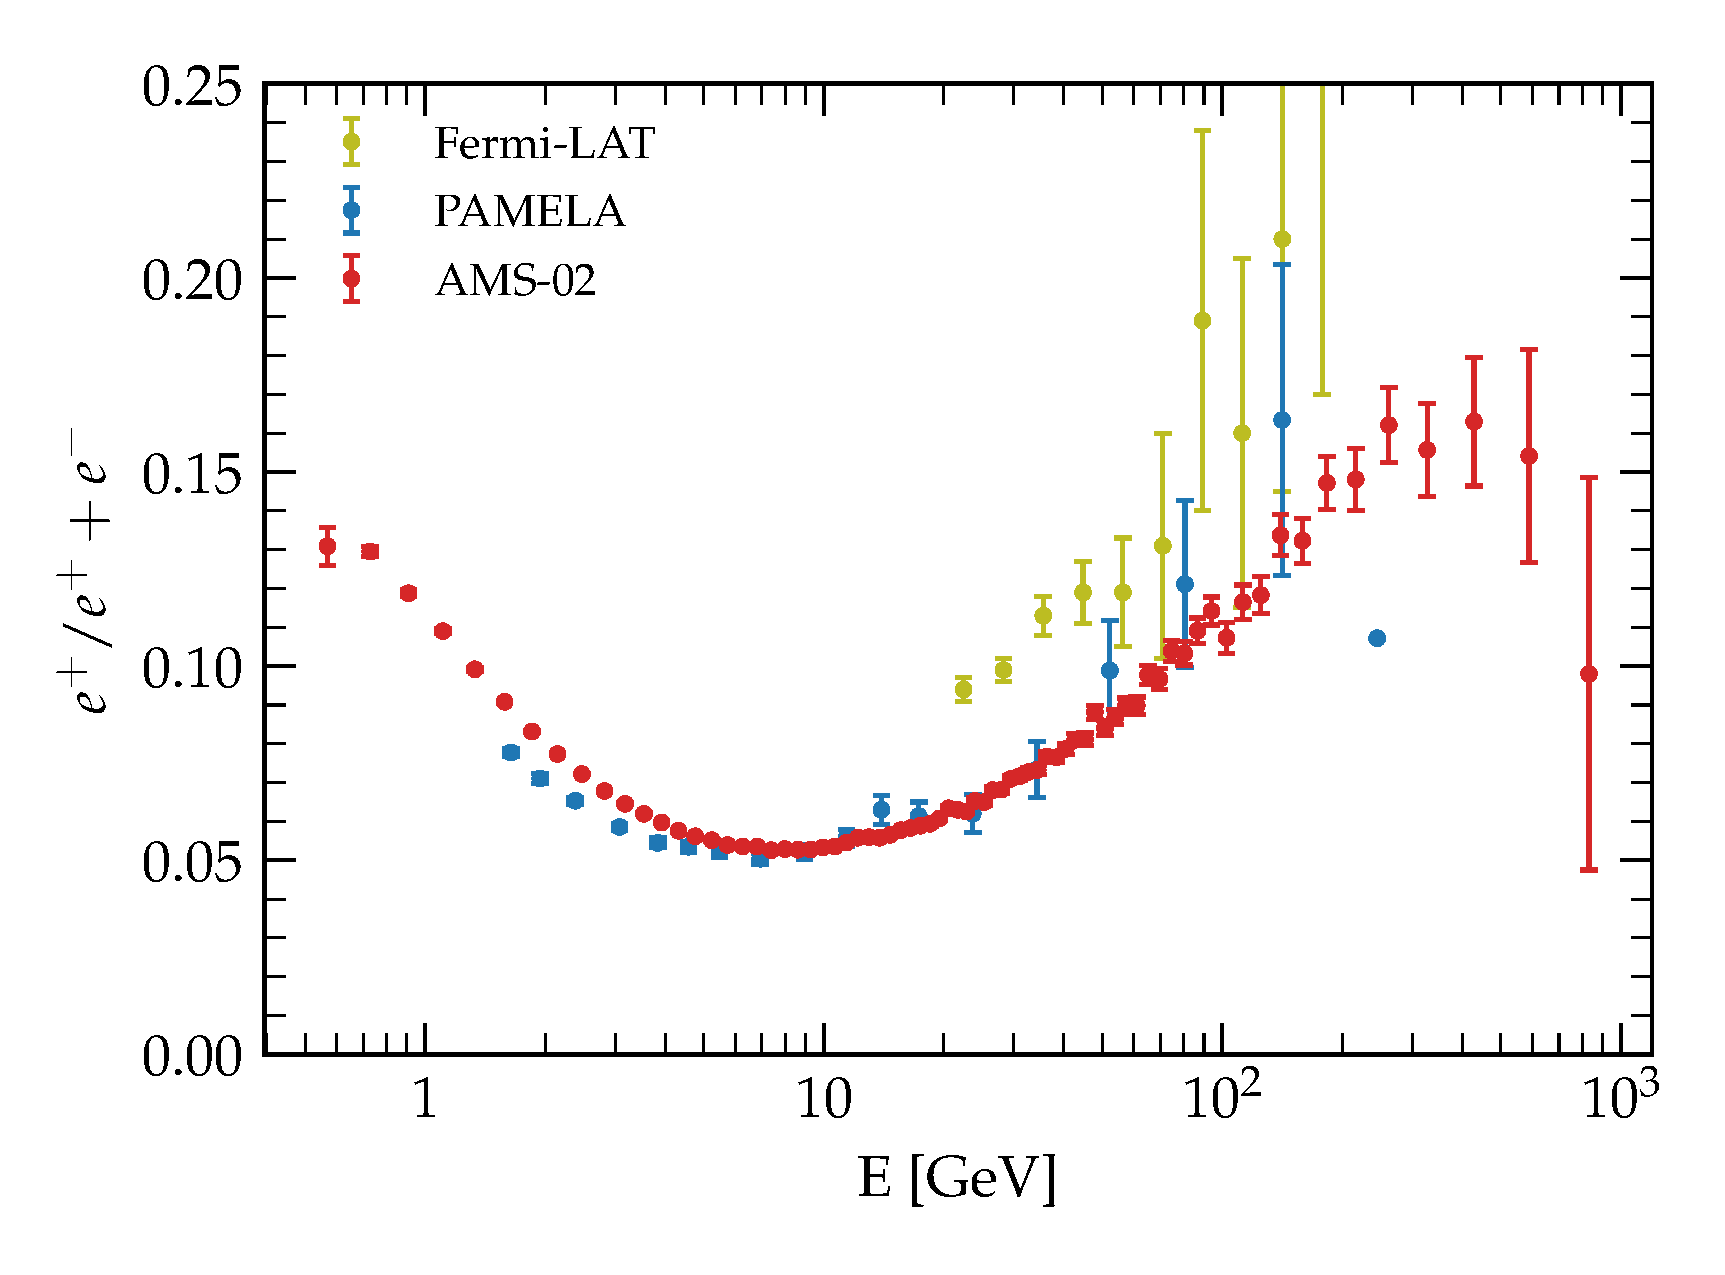
\includegraphics[width=0.6\textwidth]{figures/positron_fraction.pdf}
\caption{The positron fraction as a function of electron or positron energy as measured by PAMELA, FERMI, and AMS-02~\cite{PAMELA.2009.posfraction,FERMI.2012.posfraction,AMS02.2013.posfraction}.}
\label{fig:positronfraction}
\end{figure}

It is interesting to apply this model to compute secondary electrons and positrons.

Secondary positrons are primarily produced through nuclear reactions between protons in the cosmic radiation and protons in the target gas, resulting in the production of charged pions ($\pi^\pm$) and other mesons, with positrons being one of the final products of the decay chain.

Typically, the energy of secondary positrons is a fraction $\xi \sim \mathcal{O}(5\%)$ of the parent proton energy $E_p$:
%
\begin{equation}
E_{e^+} \simeq \xi E_p 
\end{equation} 

The rate of positron ($e^+$) production in the ISM can be expressed as:
%
\begin{equation}
q_{e^+}(E) dE = n_p(E_p) dE_p \sigma_{\rm pp} c 2 h_d n_{\rm d} \delta(z) 
\label{eq:positronproduction}
\end{equation}

Applying the solution of equation~\eqref{eq:leptonprop}, when losses are unimportant, we obtain:
%
\begin{equation}
f_{e^+}(E) = 
n_p\!\left(\frac{E}{\xi} \right) \frac{2 c \sigma_{\rm pp} n_d h_d}{\xi}  \frac{H}{D(E)} 
%\frac{N_p(E/\xi) \mathcal R_{\rm SN}}{2\pi R_d^2} \frac{H}{D(E+)}  \frac{1}{\xi} n_d h_d \sigma_{\rm pp} c \frac{H}{D(E)}
\end{equation}

Whereas, in the limit where losses dominate, equation~\eqref{eq:leptonsolution}, we have:
%
\begin{equation}
f_{e^+}(E) = 
n_p\!\left(\frac{E}{\xi} \right) \frac{2 c \sigma_{\rm pp} n_d h_d}{\xi}  \frac{\tau_{\rm loss}(E)}{\sqrt{\tau_{\rm loss}(E) D(E)}} 
%\frac{N_p(E/\xi) \mathcal R_{\rm SN}}{2\pi R_d^2} \frac{H}{D(E+)}  \frac{1}{\xi} n_d h_d \sigma_{\rm pp} c \frac{H}{D(E)}
\end{equation}

It is worth noting that the proton spectrum is always evaluated at an energy $1/\xi$ larger than the positron energy.

In both cases, one obtains:
%
\begin{equation} 
\frac{f_{e^+}}{f_{e^-}}(E) = \frac{q_{p,0}(E/\xi)}{q_{e,0}(E)} \frac{1}{\xi} \frac{\rchi(E / \xi)}{\hat\rchi} \sim E^{-\gamma_p+\gamma_e-\delta}
\label{eq:positronfractiontheory}
\end{equation}

\begin{figure}[t]
\centering
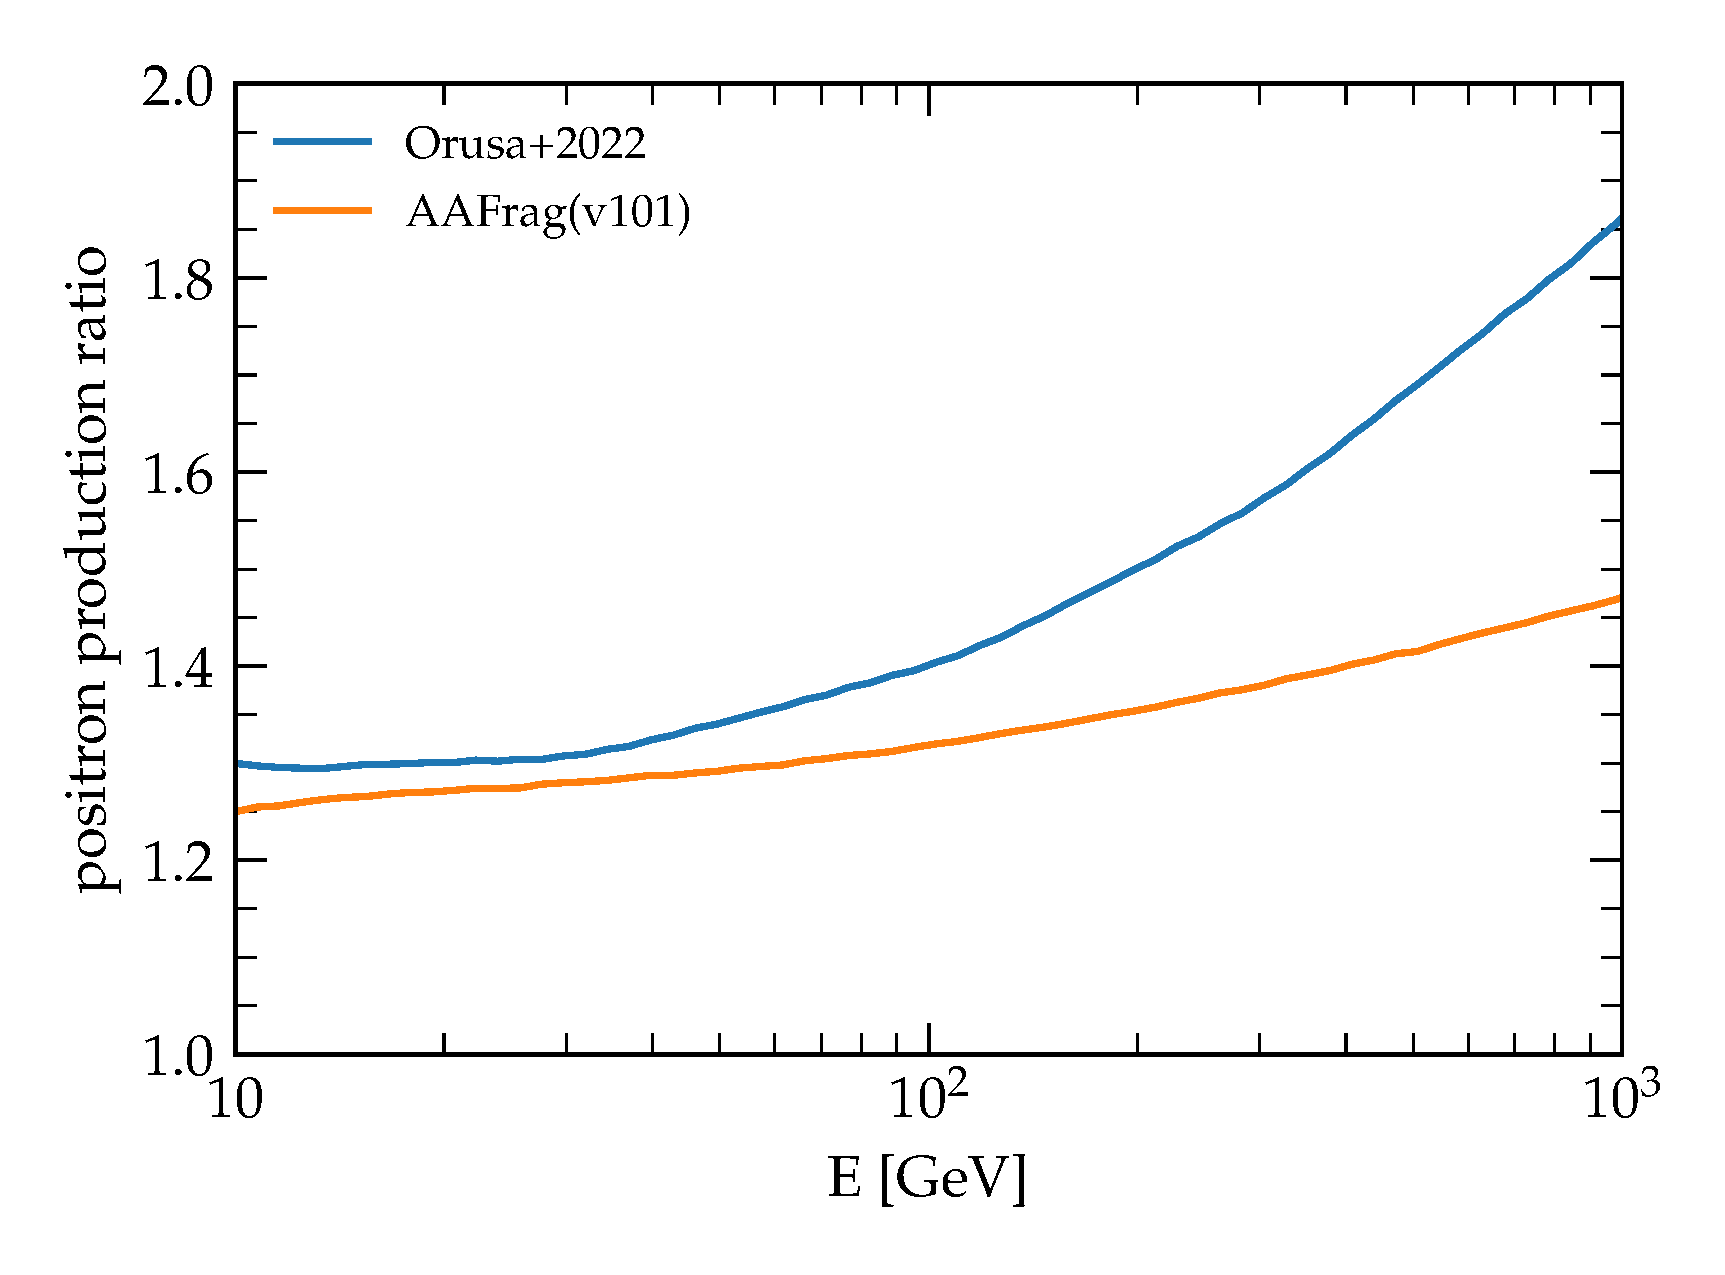
\includegraphics[width=0.6\textwidth]{figures/positron_source_term.pdf}
\caption{The positron production rate computed in two recent models~\cite{Kachelriess2019cpc,Orusa2022prd} normalized to the production rate in the constant-\emph{inelasticity} approach outlined in the text.}
\label{fig:positronsourceratio}
\end{figure}

This is different from the case of B/C, where carbon was the parent of boron,  as here electrons are not parents of secondary electrons.
%
Notwithstanding, assuming $\gamma_p \simeq \gamma_e$, the positron fraction is a decreasing function with energy, approximately following $E^{-\delta}$.

In figure~\ref{fig:positronfraction}, we present the positron fraction as a function of energy, which markedly deviates from the expectation for pure secondary production above $\sim$10 GeV.

Following equation~\eqref{eq:positronfractiontheory}, for the positron fraction to increase with energy, it would require $\gamma_e > \gamma_p + \delta$, which is highly unlikely!

Another possibility we may consider to explain the anomaly in the positron fraction is a significant modification of the cross-sections involved in secondary production processes.
%
Recent efforts have been made to re-evaluate these cross-sections by fitting data from collider experiments or by utilizing hadronic interaction models~\cite{Orusa2022prd,Kachelriess2019cpc}. The production rates obtained using these approaches can be compared with the rates predicted by equation~\eqref{eq:positronproduction}, as shown in figure~\ref{fig:positronsourceratio}. 
%
The comparison reveals that there are no deviations from our initial naive approach at a level that would account for the observed excess.

As such, we are left with no other option than to postulate the existence of a new population of positron sources in the Universe!
